\documentclass{beamer}
\usepackage[english,russian]{babel}
\usepackage[utf8]{inputenc}
%\usepackage{smaller}
\usepackage{multicol}
\usepackage{tabularx}
\usepackage{wasysym}

%biblatex-gost
\usepackage[backend=biber, style=gost-authoryear, bibstyle=gost-authoryear, language=auto, babel=other, bibencoding=utf8, bibdoi=false, biburl=false,  movenames=false, sortcites = false]{biblatex}
\addbibresource{../txt/sophia_base.bib}


\mode<presentation>
%\mode<article>
% Стиль презентации
%\usetheme{Warsaw}
% \usetheme{Madrid}
\usetheme{Marburg}
%\usetheme{Hannover}
%\usetheme{Singapore}
%\usecolortheme{seahorse}



% в начале каждого раздела печатаем содержание с выделением текущего раздела
%\AtBeginSection[]
%{
%  \begin{frame}<beamer>{Содержание}
%    \tableofcontents[currentsection]
%  \end{frame}
%}




\begin{document}

\title[]{ОРГАНИЗАЦИЯ ПОСЕЛЕНИЙ\\ {\it Macoma~balthica}~(Linnaeus,~1758)\\ В ОСУШНОЙ ЗОНЕ БЕЛОГО И БАРЕНЦЕВА МОРЕЙ}
\author[]{София Александровна Назарова \\ \medskip
	\footnotesize{Научный руководитель: д.б.н.~Н.~В.~Максимович}}
\institute[СПбГУ]{Санкт-Петербургский государственный университет}
\date{Санкт-Петербург, 2015} 

% Создание заглавной страницы
\frame{\titlepage} 



% Автоматическая генерация содержания
%\frame{\frametitle{Содержание}\tableofcontents} 


%%%%%%%%%%%%%%%%%%%%%%%%%%%%%%%%%%%%%%%%%%%%%%%%%%%%%
		\section{Введение}
%%%%%%%%%%%%%%%%%%%%%%%%%%%%%%%%%%%%%%%%%%%%%%%%%%%%%
\begin{frame}{Вид {\it Macoma~balthica} (L., 1758)}
			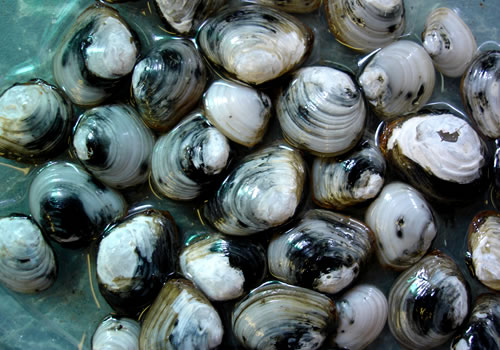
\includegraphics[width=.49\textwidth]{Baltic_macoma.jpg}	%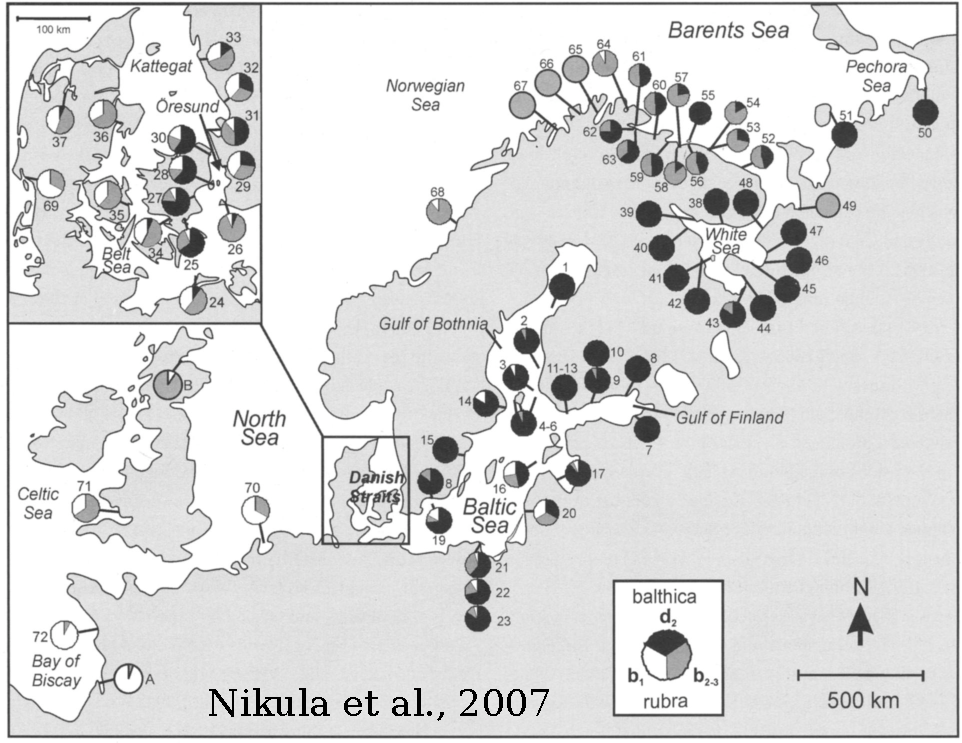
\includegraphics[width=.49\textwidth]{Macoma_genetic.pdf}

			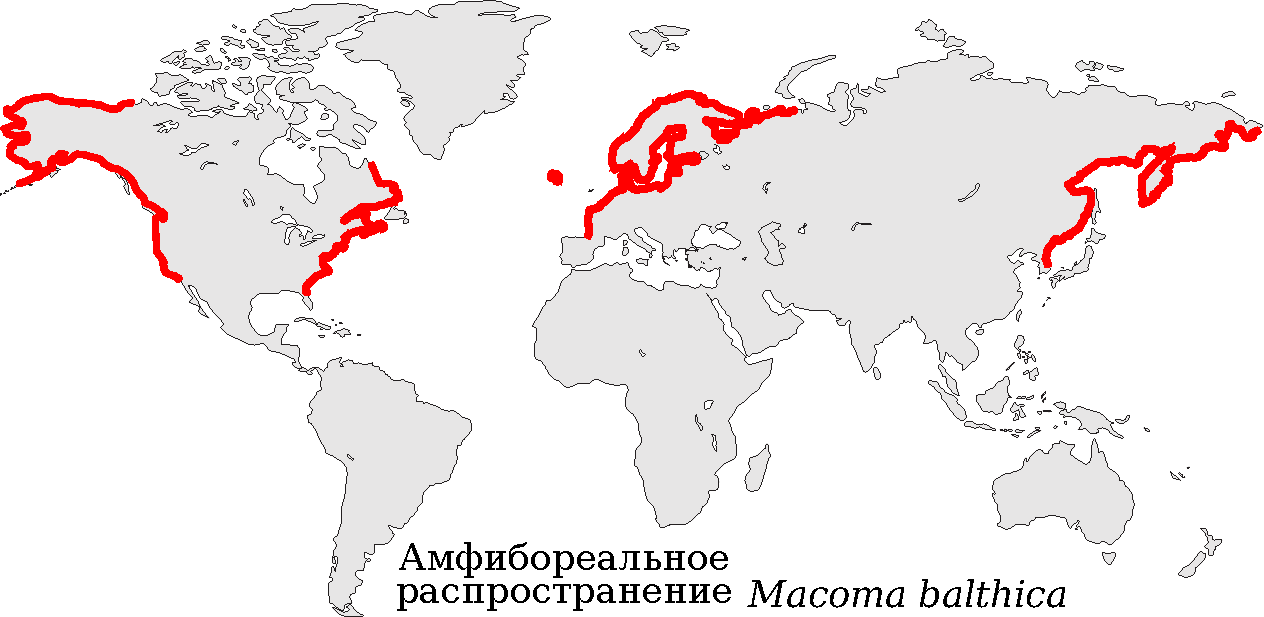
\includegraphics[width=.9\textwidth]{areal_line.pdf}


\end{frame}

\begin{frame}{Цели и задачи}
\begin{description}
	\item[Цель.] Изучение организации поселений {\it Macoma balthica} в условиях осушной зоны Белого и Баренцева морей.

	\item[Задачи.]
Для этого были изучены следующие стороны организации поселений:
  \begin{enumerate}
    \item биотический и абиотический фон биотопов;
    \item структурные характеристики поселений \textit{M.~balthica} (показатели обилия, размерная структура);
    \item многолетняя динамика поселений \textit{M.~balthica};
    \item скорость линейного роста моллюсков;
    \item режим формирования спата.
  \end{enumerate}
\end{description}
\end{frame}


\begin{frame}{Положения, выносимые на защиту}
\begin{small}
%\begin{tiny}
\begin{enumerate}
\item На литорали Кандалакшского залива Белого моря и в Баренцевом море (Западный Мурман и Кольский залив) \textit{Macoma balthica} формирует поселения, в которых плотность значительно варьирует во времени и может достигать нескольких тысяч экз./м$^2$, но наиболее типичны поселения маком с плотностью в несколько сотен экз./м$^2$. На литорали Восточного Мурмана Баренцева моря вид не формирует плотных поселений, и значения данного показателя редко превышает 100~экз./м$^2$.

\item Организация поселений  \textit{Macoma balthica} в условиях осушной зоны Белого и Баренцева морей не имеет принципиальных различий:
	\begin{itemize}
	\begin{scriptsize}
		\item  в типичном случае в многолетней динамике поселений сменяются мономодальный (преобладание молоди) и бимодальной (добавление второго модального класса~--- группы особей старшего возраста) типы размерной структуры; 
		\item как относительно редкое событие наблюдаются мономодальная структура поселений с ежегодным преобладаем молоди.
	\end{scriptsize}
	\end{itemize}

\end{enumerate}
\end{small}
%\end{tiny}
\end{frame}


\begin{frame}{Положения, выносимые на защиту}
%\begin{scriptsize}
%\begin{tiny}
\begin{enumerate}
\addtocounter{enumi}{2}

\item Характер динамики плотности поселений \textit{Macoma balthica} определяется, в основном, неравномерностью  уровня ежегодного пополнения их молодью. 
Беломорские поселения демонстрируют элементы синхронности процессов пополнения, что связано с влиянием температуры на выживаемость маком в первый год жизни  (численность однолетних особей после холодных зим с устойчивым ледоставом оказывается относительно выше) и спецификой условий в локальном местообитании.

\item Скорость роста особей \textit{Macoma balthica} в Белом и Баренцевом морях достоверно ниже, чем в других акваториях европейской части ареала вида. 
По характеру вариации средней скорости роста маком поселения Баренцева моря и Белого моря различий не имеют. 
\end{enumerate}
%\end{scriptsize}
%\end{tiny}
\end{frame}

%%%%%%%%%%%%%%%%%%%%%%%%%%%%%%%%%%%%%%%%%%%%%%%%%%%%%
		\section[Методы]{Материал и методика}
%%%%%%%%%%%%%%%%%%%%%%%%%%%%%%%%%%%%%%%%%%%%%%%%%%%%%
\begin{frame}{География исследований: Кандалакшский залив Белого моря}
 \begin{center}
	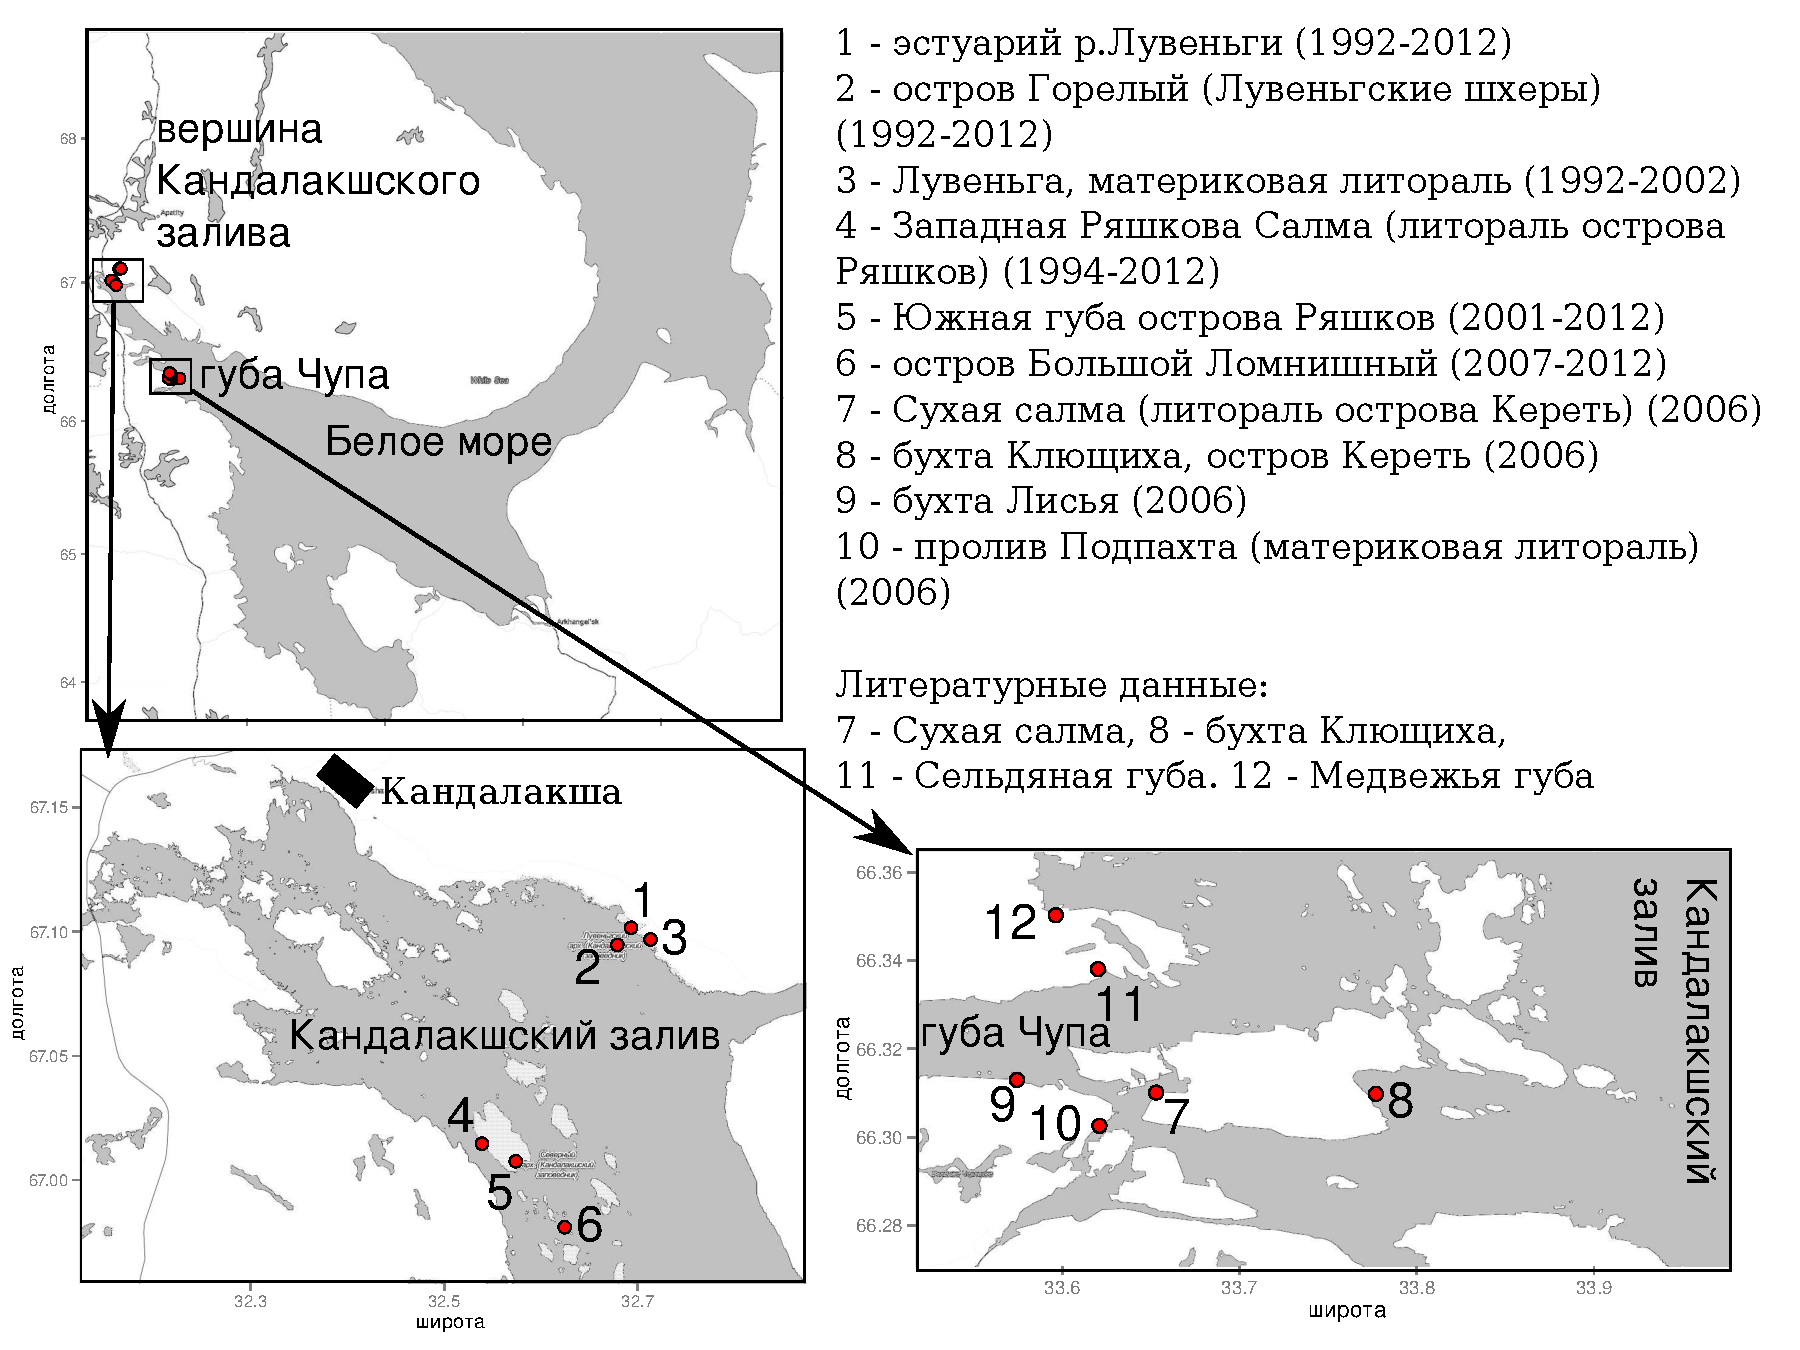
\includegraphics[height=.8\textheight]{./White_sea.pdf}
 \end{center}
\end{frame}

\begin{frame}{География исследований: Мурманское побережье Баренцева моря}
 \begin{center}
	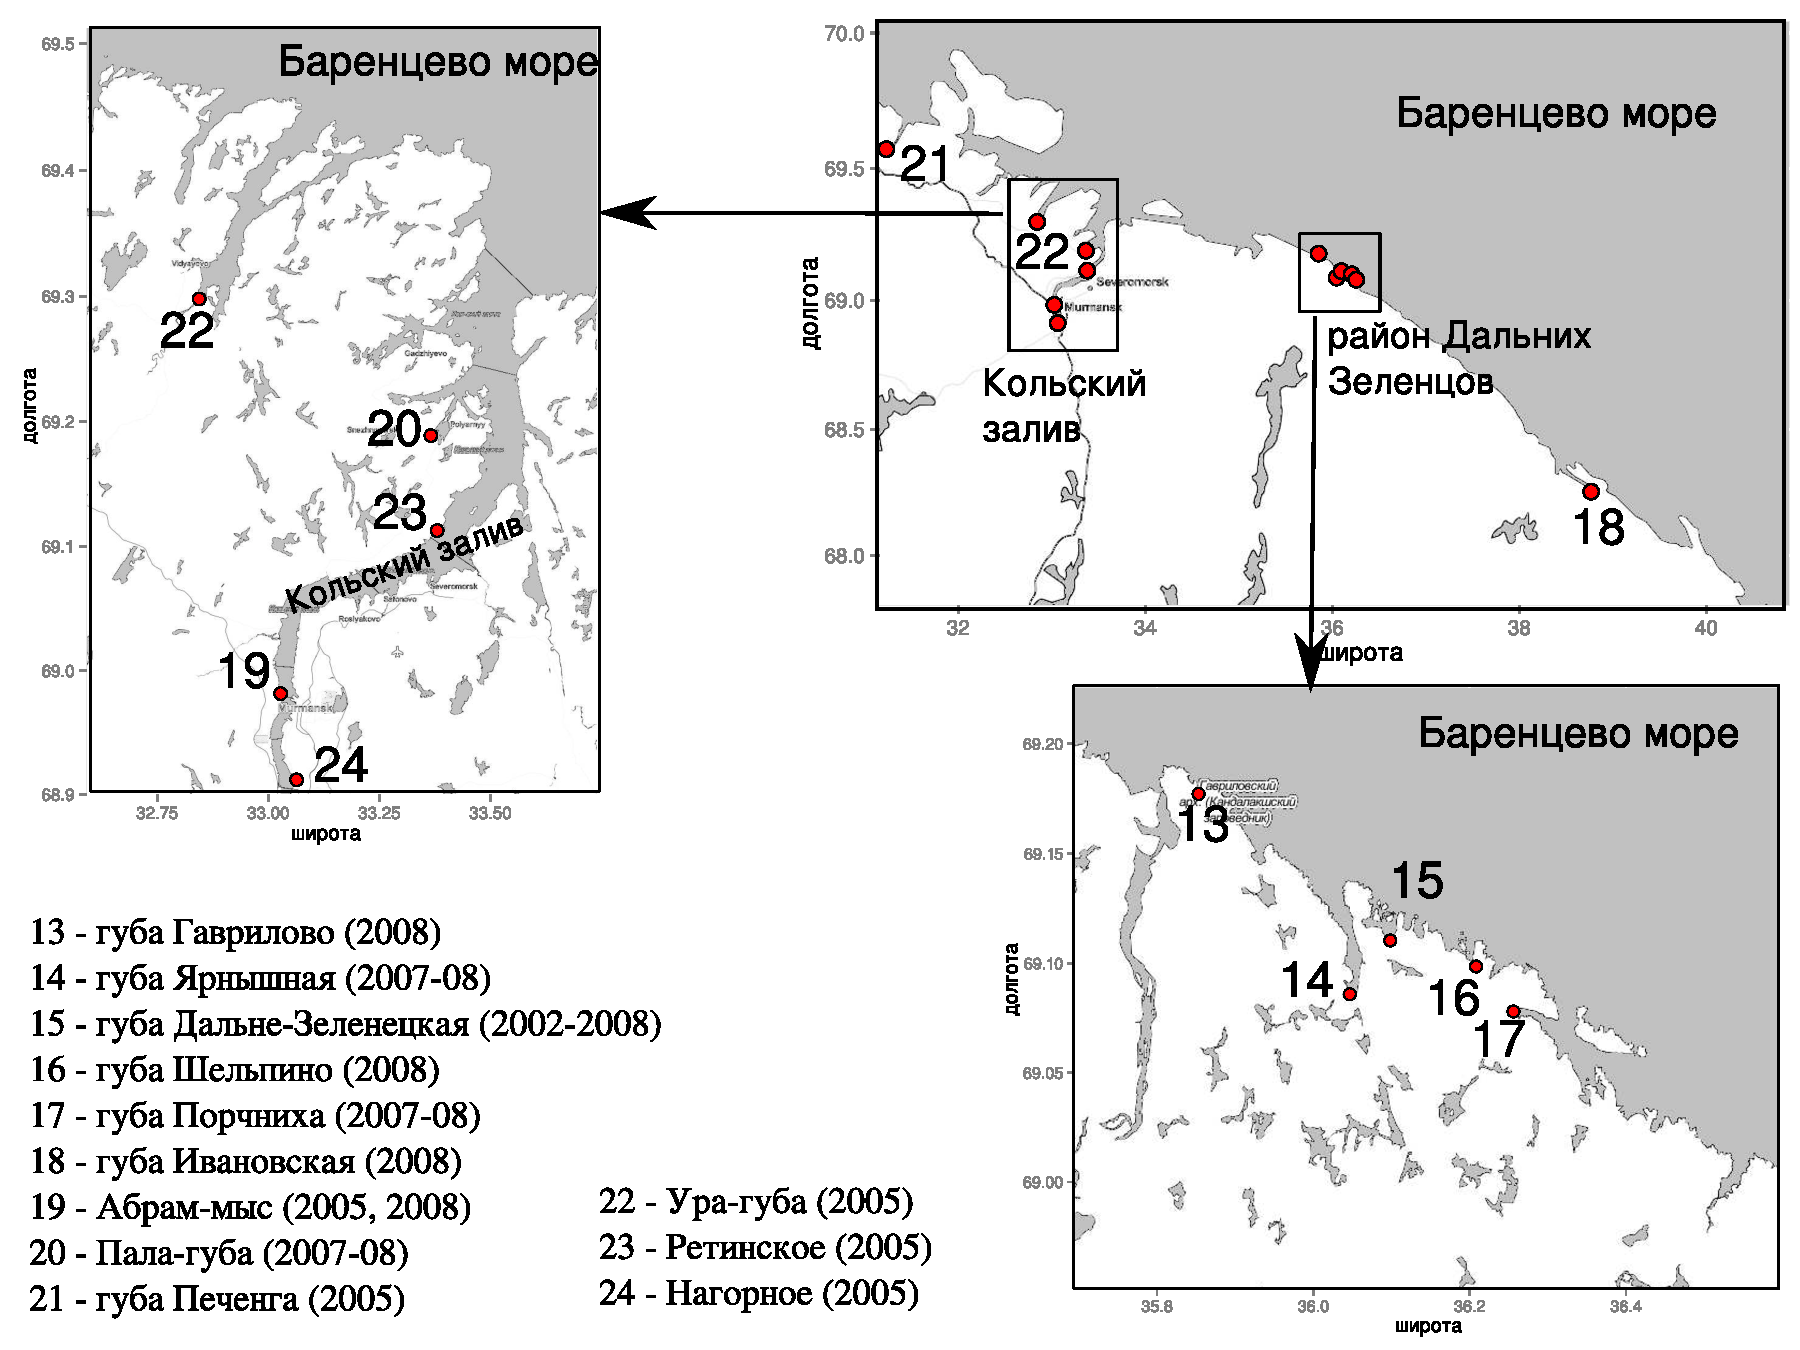
\includegraphics[height=.8\textheight]{./Barents_sea.pdf}
 \end{center}
\end{frame}

\begin{frame}{Методы: Полевые сборы}
 \begin{description}
 		\item [Пробоотборник:] Литоральные рамки площадью 1/30~м$^2$ или $3 \times$~1/30~=~1/10~м$^2$ (интегрированная проба), либо зубчатый водолазный дночерпатель площадью~1/20~м$^2$
		\item [Однократная съемка:] от 3 до 36 проб
		\item [Промывка:] сито с диаметром ячеи $1$~мм 
		\item [Обработка:] подсчет всех особей в пробах, измерение длины и меток остановки роста, взвешивание
	\end{description}
\end{frame}

\begin{frame}{Методы: Описание биотопов}
	\begin{minipage}[c]{.3\linewidth}
		\begin{center}
%		{\footnotesize Белое море}
			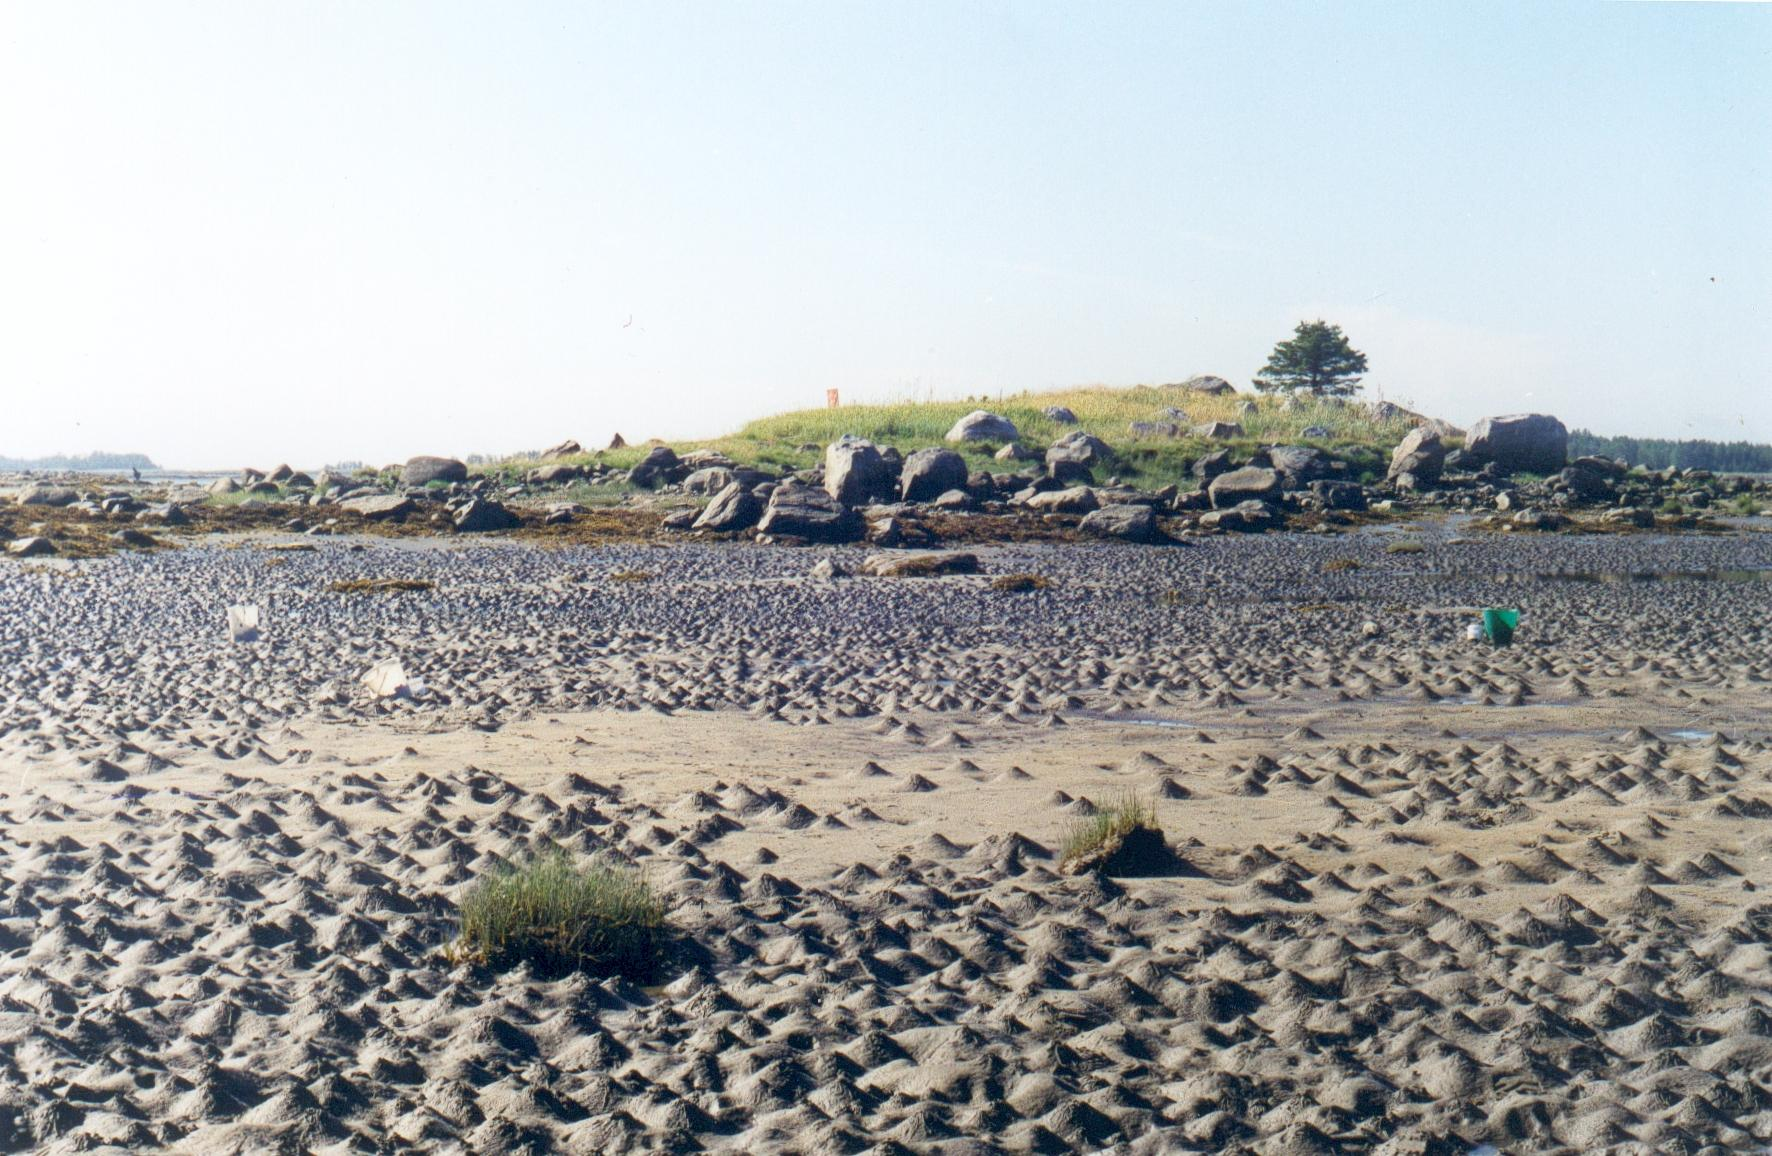
\includegraphics[width=\textwidth]{Luvenga_Estuary.JPG}\\
			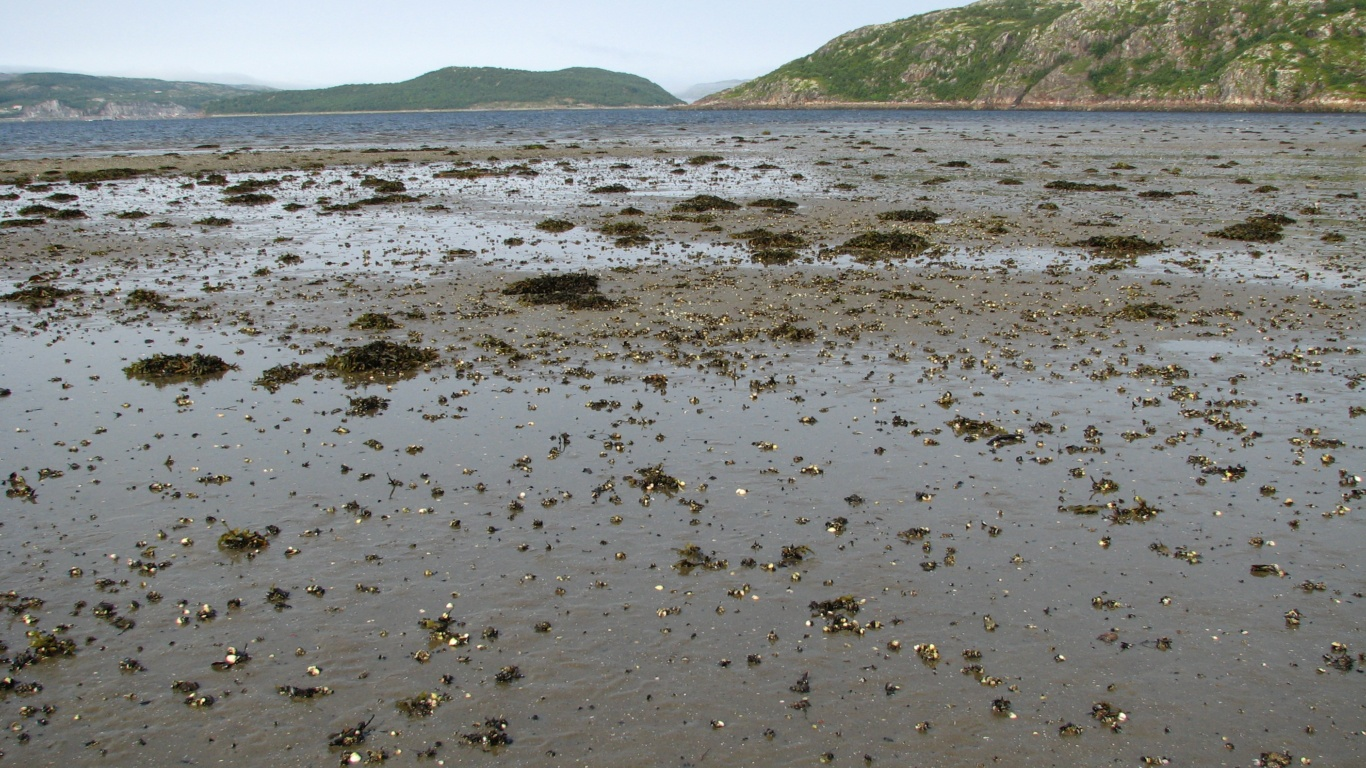
\includegraphics[width=\textwidth]{Ura.JPG} \\
			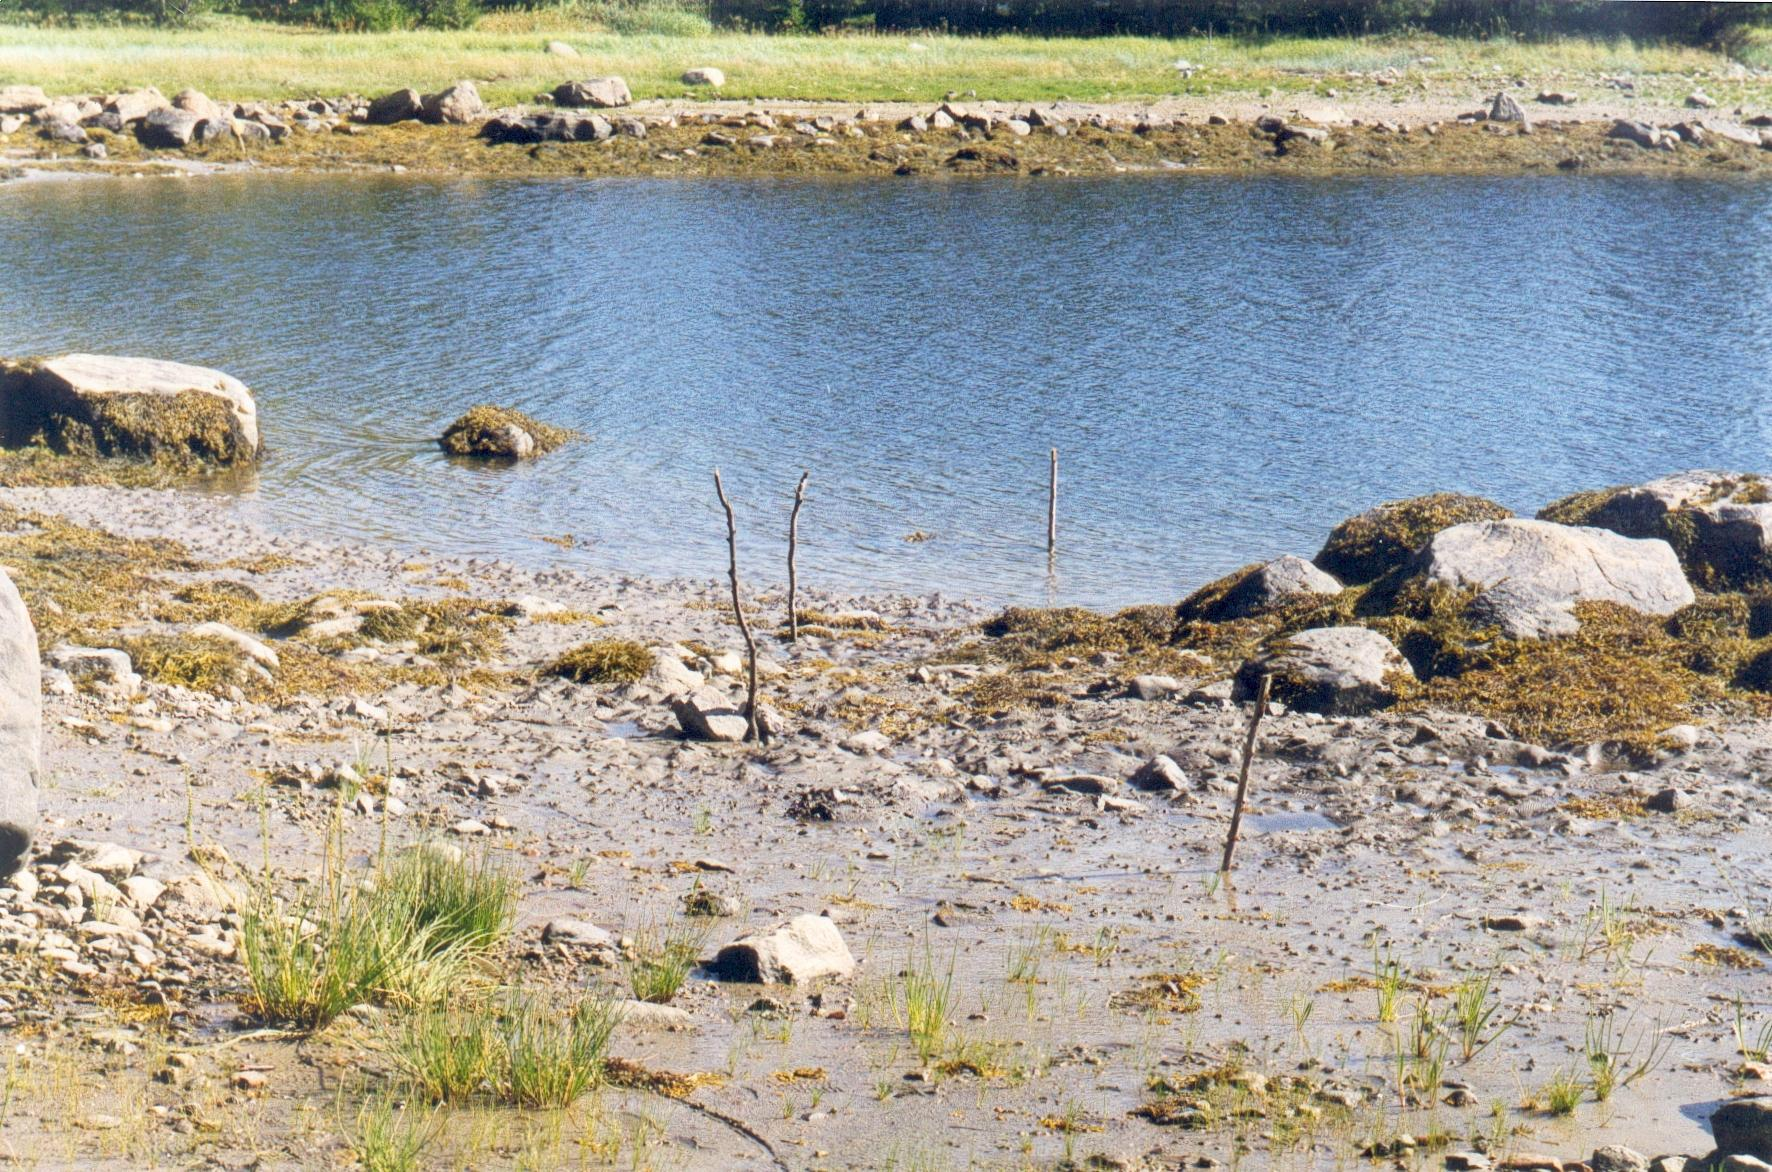
\includegraphics[width=\textwidth]{Goreliy.JPG} \\
			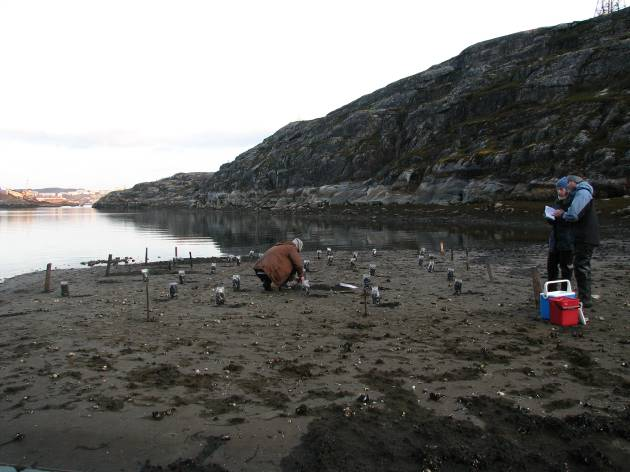
\includegraphics[width=\textwidth]{Pala.JPG}
		\end{center}
	\end{minipage}
	\begin{minipage}[c]{.60\linewidth}
\begin{small}
 \begin{description}
%	\item [Визуальное описание:] \\ширина литорали, визуально тип грунта, наличие валунов, бурых водорослей, взморника Zostera marina, зеленых нитчатых водорослей.

	\item[Грунт:] 

гранулометрический состав, содержание органических веществ

	\item[Биотический фон:] Описание таксономического состава

	\item[Температурный режим:] по данным Летописи природы Кандалакшского заповедника (1991 - 2000), Архива погоды в Кандалакше (2014), декадной станции ББС <<Картеш>> и разреза <<Кольский меридиан>>. 
  \end{description}
\end{small}

%		\begin{center}
%		{\footnotesize Белое море}
%			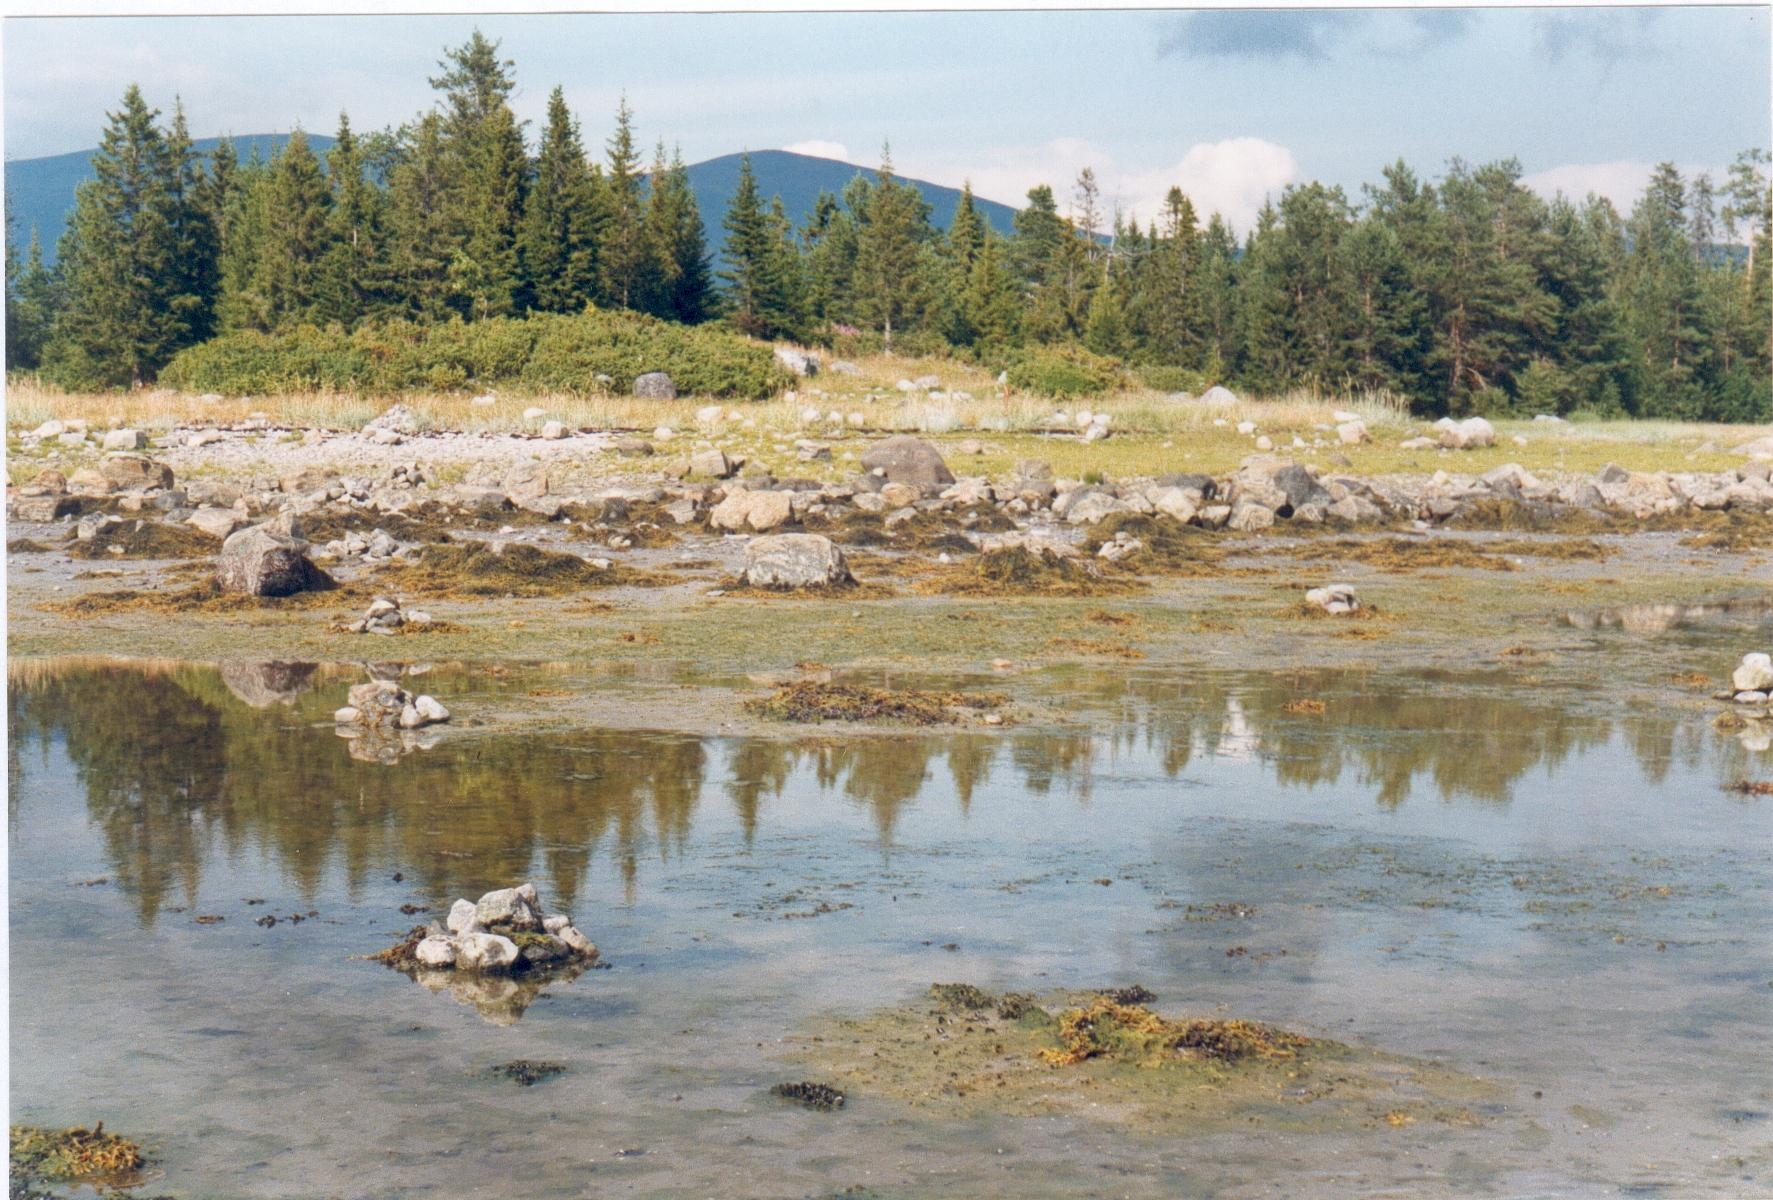
\includegraphics[width=\textwidth]{razrez2.JPG} \\
%			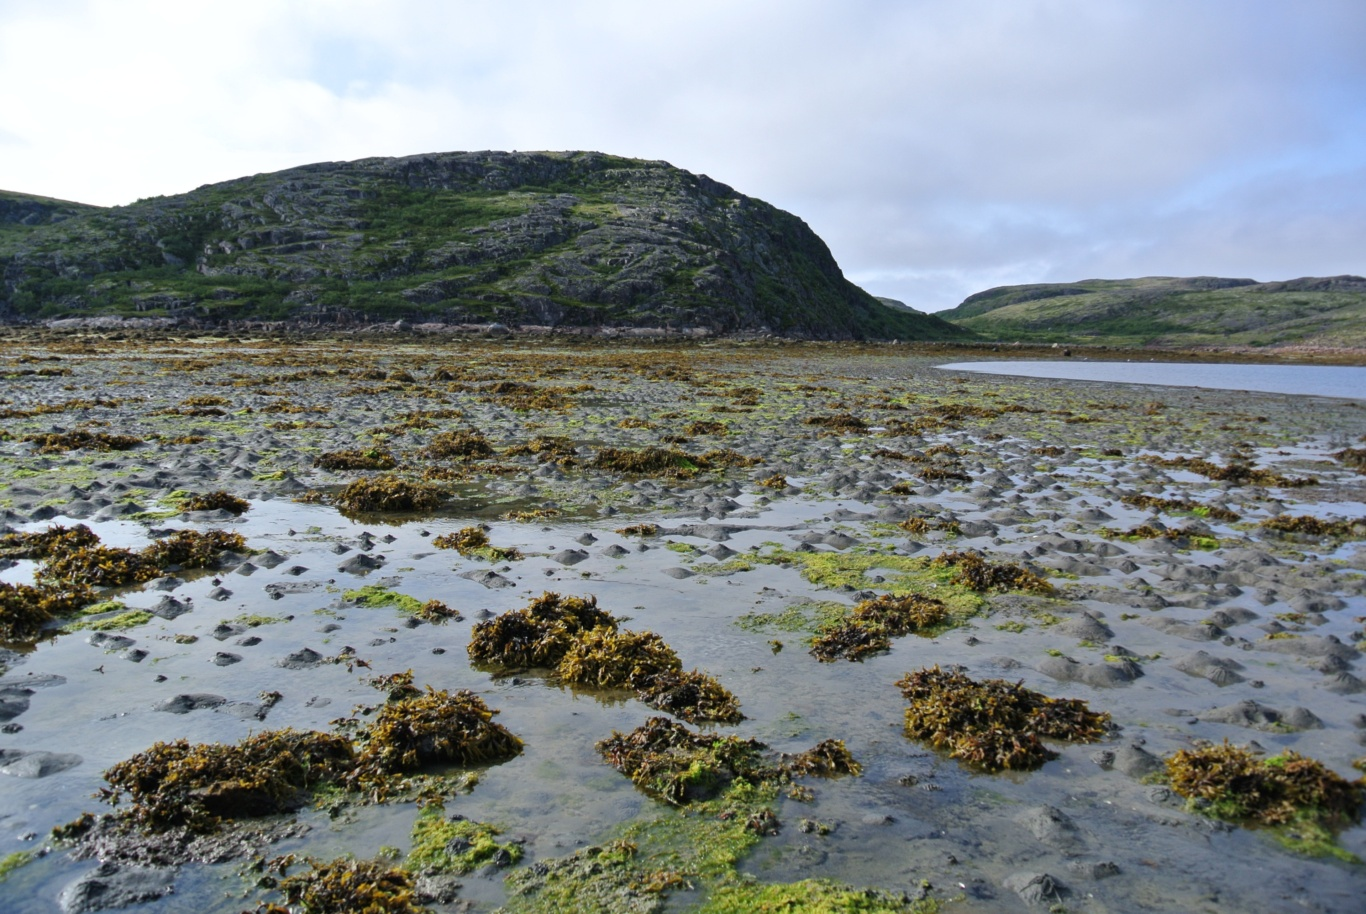
\includegraphics[width=\textwidth]{Yarnyshka.jpg}
%		\end{center}
	\end{minipage}
%			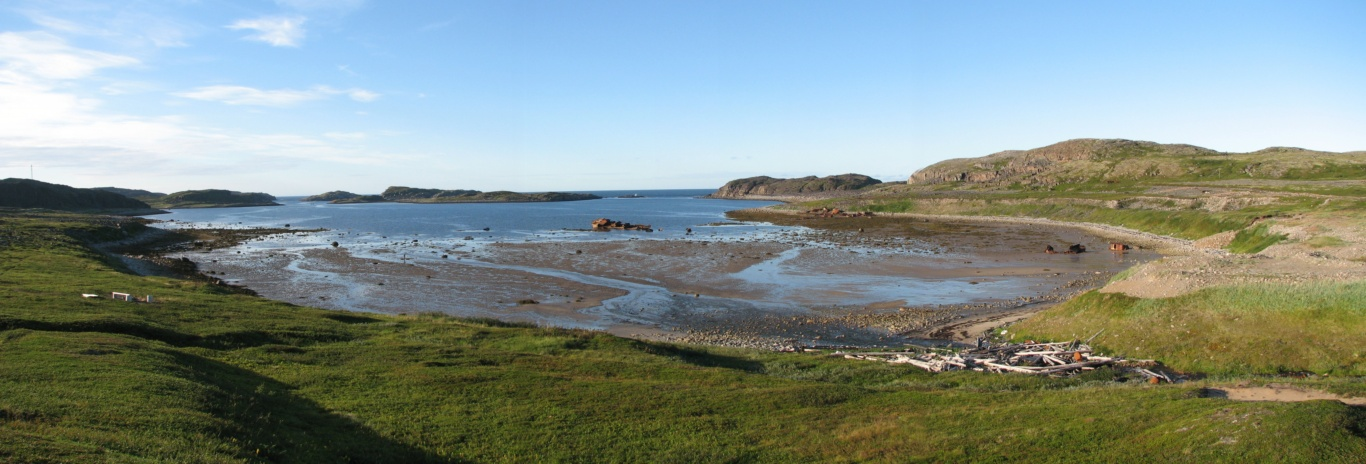
\includegraphics[width=\textwidth]{DZ.jpg}
\end{frame}

\begin{frame}{Методы: Структурные характеристики}
 \begin{description}
	\item [Показатели:] Средняя плотность поселения, средняя биомасса поселения, размерная структура поселения.
	\item [Получение данных:] 
		\begin{itemize}
			\item Прямое наблюдение
			\item Для части участков на Белом море биомассу определяли расчетным методом (Максимович и др., 1993).
		\end{itemize}
	\item [Анализ:] 
		\begin{itemize}
			\item Сравнение поселений по среднему обилию проводили с помощью непараметрического теста Краскела-Уоллиса.
			\item Сравнительный материал: информация о средних плотности поселения и биомассе в европейской части ареала вида.
		\end{itemize}	
\end{description}
\end{frame}

\begin{frame}{Методы: Динамика поселений}
\begin{small}
 \begin{description}
	\item [Показатели:] Плотность поселений, размерная структура поселения, плотность поселений однолетних маком (пополнение).
	\item [Материал:] 
		\begin{itemize}
			\item Мониторинг 6 поселений маком в вершине Кандалакшского залива и 1~--- на Восточном Мурмане: длина рядов от 7 до 20 лет.
			\item 4 поселения в районе губы Чупа Белого моря (Максимович и др.,1991; Gerasimova, Maximovich, 2013; Varfolomeeva, Naumov, 2013): длина рядов от 21 до 27 лет.
		\end{itemize}
	\item [Анализ:] 
		\begin{itemize}
			\item Попарное сравнение динамики плотности поселений в Белом море с помощью корреляции Мантеля.
			\item Линейная модель зависимости динамики плотности поселений  от температуры.
		\end{itemize}
\end{description}
\end{small}
\end{frame}

\begin{frame}{Методы: Линейный рост}
\begin{small}
 \begin{description}
	\item [Материал:] 
		\begin{itemize}
			\item 7 Баренцевоморских поселений маком: 2 в Кольском заливе, 5 на Восточном Мурмане.
			\item Сравнительный материал: ростовые характеристики {\it M.~balthica} в европейской части ареала (25 поселений).
		\end{itemize}
	\item [Данные:] Описание роста особей по меткам зимних остановок роста.
	\item [Анализ:] 
		\begin{itemize}
			\item Аппроксимация уравнением Берталанфи: $L_{t} = L_{max} \times (1 - e^{(-k(t - t_{0}))})$, где $L_{max}$, $k$, $t_{0}$~--- коэффициенты, а $L_{t}$~--- длина раковины моллюска в возрасте $t$.
			\item Сравнение кривых роста с учетом разброса эмпирических данных относительно регрессионной модели (Максимович, 1989).
			\item Широтные изменения скорости роста анализировали, сравнивая КПД роста $\omega = L_{max} \times k$ .
		\end{itemize}
\end{description}
\end{small}
\end{frame}


\begin{frame}{Методы: Формирование спата}
\begin{small}
 \begin{description}
	\item [Материал:] 4 Беломорских поселения в районе Керетского архипелага (специальные сборы в июле и сентябре 2006 года).
	\item [Данные:] Структура сообщества макрозообентоса (площадь учета 1/10 м$^2$) и плотность поселения спата (площадь учета 1/100 м$^2$).
	\item [Анализ:] Иерархический дисперсионный анализ: влияние обилия маком, обилия макрозообентоса и участка на плотность поселения спата.
%		\begin{itemize}
%			\item 
%		\end{itemize}
\end{description}
\end{small}
\end{frame}

%%%%%%%%%%%%%%%%%%%%%%%%%%%%%%%%%%%%%%%%%%%%%%%%%%%%%
		\section[Биотопы]{Биотический и абиотический фон биотопов}
%%%%%%%%%%%%%%%%%%%%%%%%%%%%%%%%%%%%%%%%%%%%%%%%%%%%%
\begin{frame}{Условия обитания \textit{Macoma balthica} в Белом и Баренцевом морях}
\begin{scriptsize}
%\begin{small}
\begin{tabularx}{\textwidth}{|p{0.2\textwidth}|X|XX|} \hline
		& Белое море		    & \multicolumn{2}{c|}{Баренцево море:} \\
показатель	&	Кан\-да\-лакш\-ский залив &	Мурманское побережье & Кольский залив	\\ \hline \hline
\multicolumn{4}{|c|}{ТЕМПЕРАТУРА ВОДЫ:} \\ \hline 
min, $^{\circ}C$	&	{\large -1.5}	&	\multicolumn{2}{c|}{{\large3 -- 5}}  	\\
max, $^{\circ}C$	&	{\large15 (до 20)}	&	\multicolumn{2}{c|}{{\large8 (до 18)}}		\\ \hline \hline
\multicolumn{4}{|c|}{ГИДРОЛОГИЧЕСКАЯ СЕЗОННОСТЬ:} \\ \hline
макс. прогрев	& {\large лето}	&	\multicolumn{2}{c|}{{\large осень}}		\\
мин. прогрев	&	{\large зима}	&	\multicolumn{2}{c|}{{\large весна}}		\\ \hline \hline
\multicolumn{4}{|c|}{СОЛЕНОСТЬ:} \\ \hline
средне\-годовая, \permil &	{\large 23 -- 25}	&	{\large 34}	&	{\large 28}	\\
min, \permil &	{\large 10}	&	{\large 28}	&	{\large 2}	 \\ \hline \hline
про\-дол\-жи\-тель\-ность ле\-дос\-тава, мес.	&	{\large 5 -- 7} 	& \multicolumn{2}{c|}{{\large 0}, припай в отдельных губах}		\\ \hline
%высота приливной волны, м	&	3	&	4		\\ \hline
\end{tabularx}
\end{scriptsize}
%\end{small}
{\tiny (По: Дерюгин, 1915; Гурьянова и др., 1928 -- 1920; Кузнецов, 1960; Бабков, Голиков, 1984; Berger et al., 2003; \textit{Кольский меридиан, 2014})}
\end{frame}


%\begin{frame}{Термические характеристики исследованных акваторий}
%{\scriptsize (По: Berger et al., 2003; \textit{Кольский меридиан, 2014})}
%		\begin{center}
%			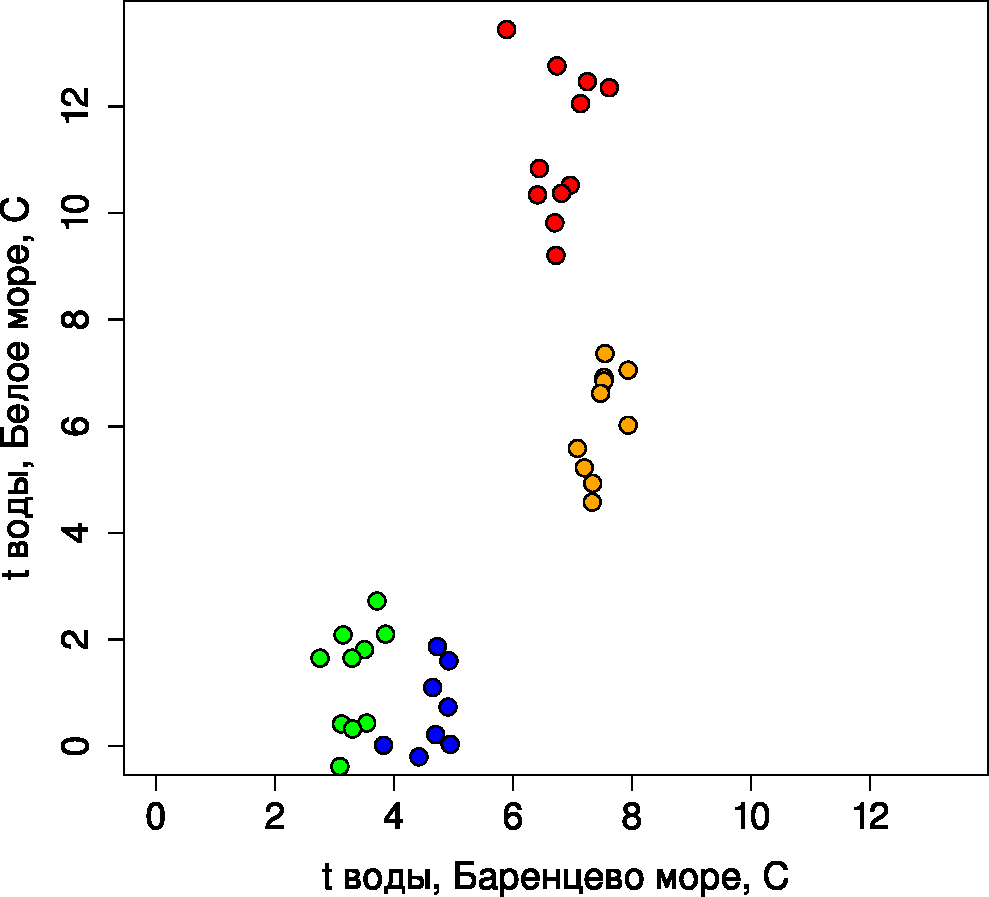
\includegraphics[width=0.65\textwidth]{temp_White_Barents_big1.pdf}
%		\end{center}
%{\scriptsize Цветовые обозначения: синий~--- зима, зеленый~--- весна, красный~--- лето, желтый~--- осень}
%\end{frame}


\begin{frame}{Гранулометрический состав грунта в исследованных биотопах}
			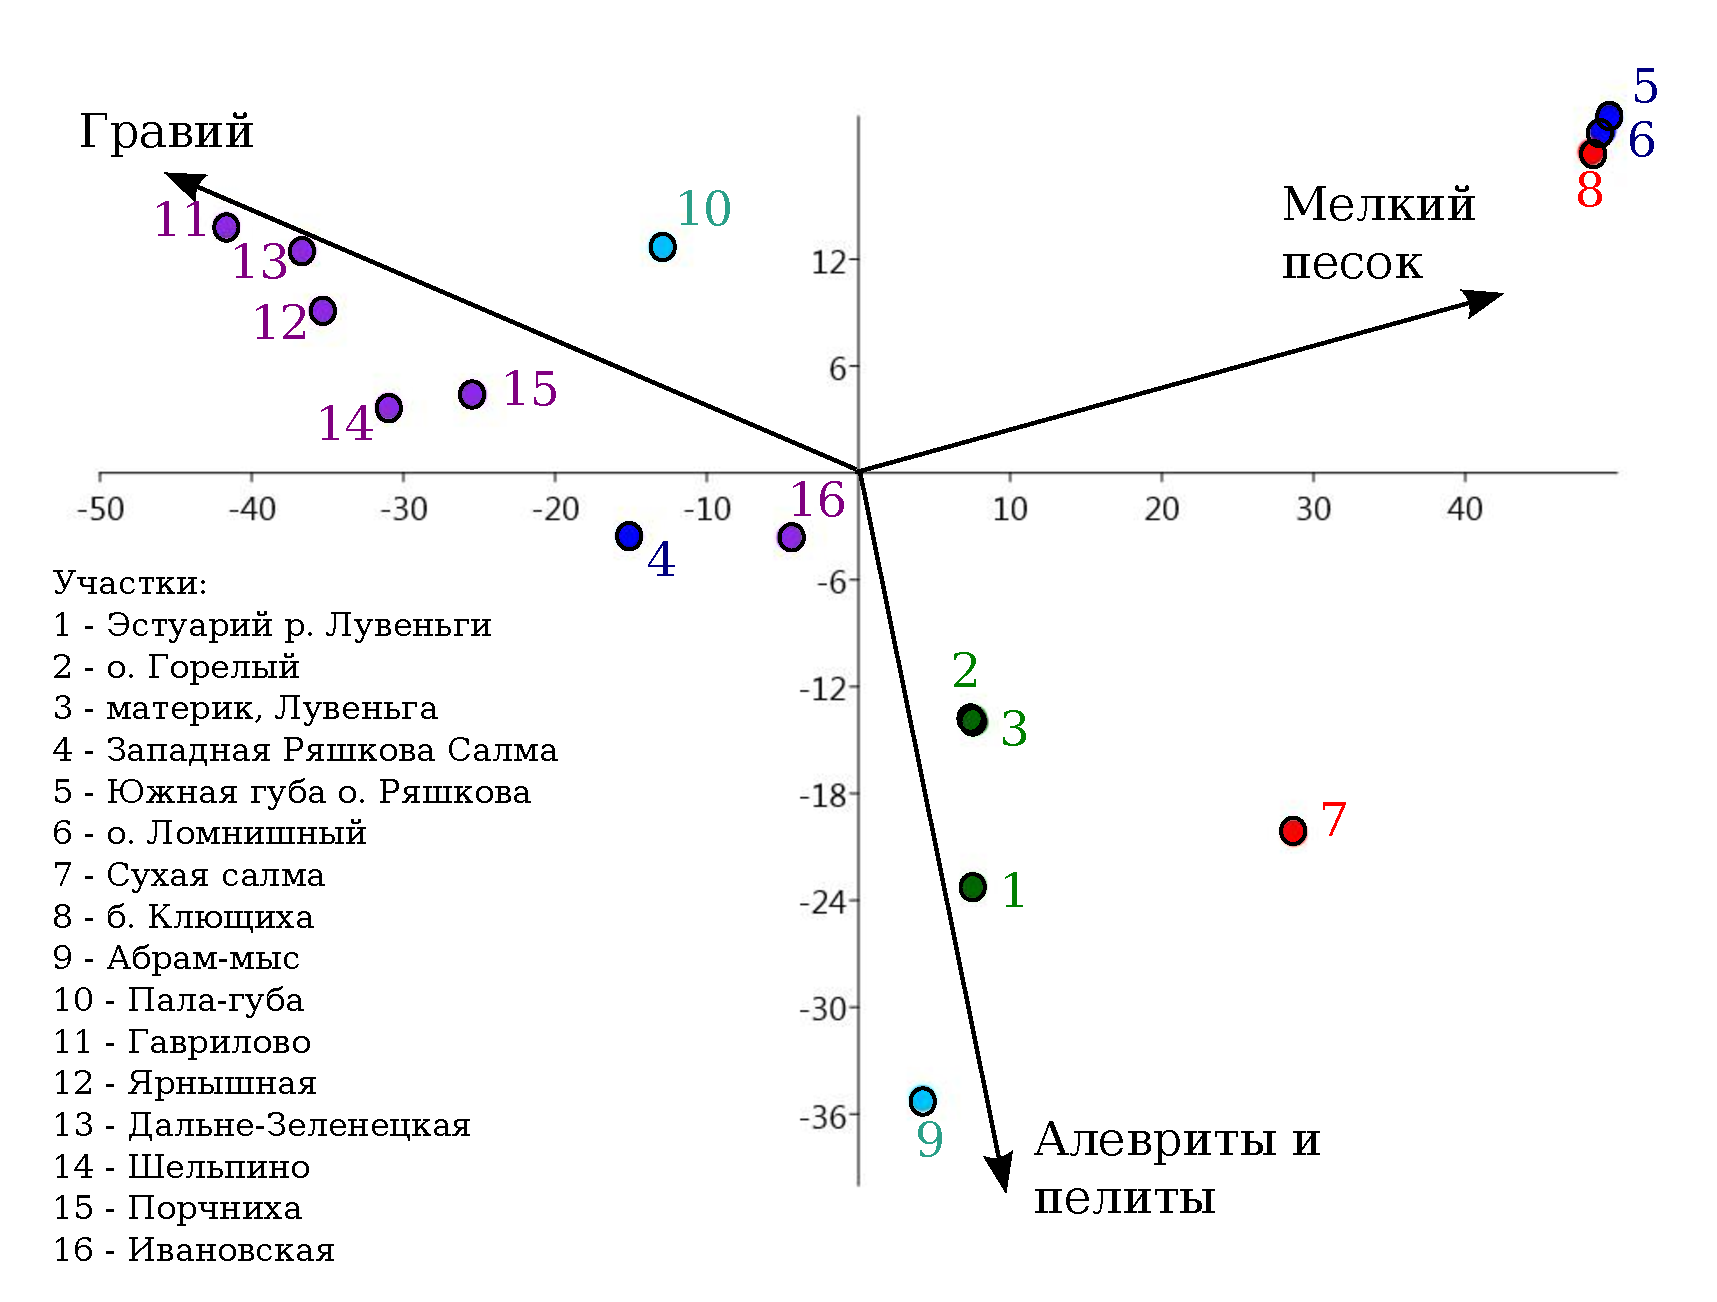
\includegraphics[width=.9\textwidth]{Grunty.pdf}
%	\begin{minipage}[t]{.49\linewidth}
%		\begin{center}
%		{\footnotesize Белое море}
%			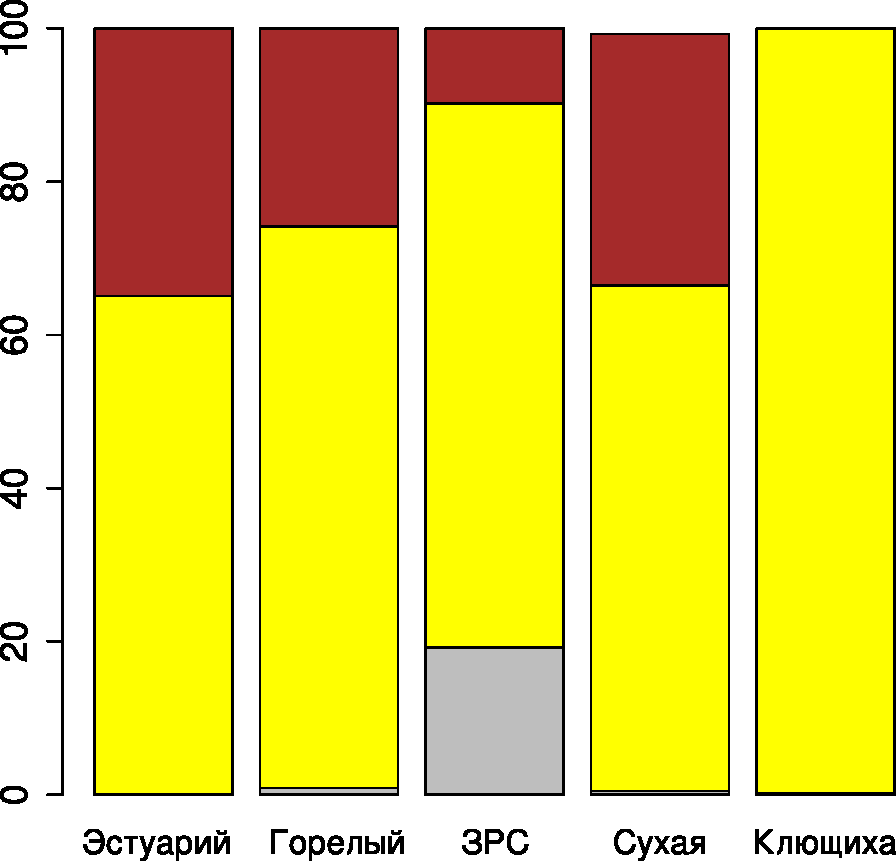
\includegraphics[width=\textwidth]{grunty_white1.pdf}
%		\end{center}
%	\end{minipage}
%
%	\begin{minipage}[t]{.49\linewidth}
%		\begin{center}
%		{\footnotesize Баренцево море}
%			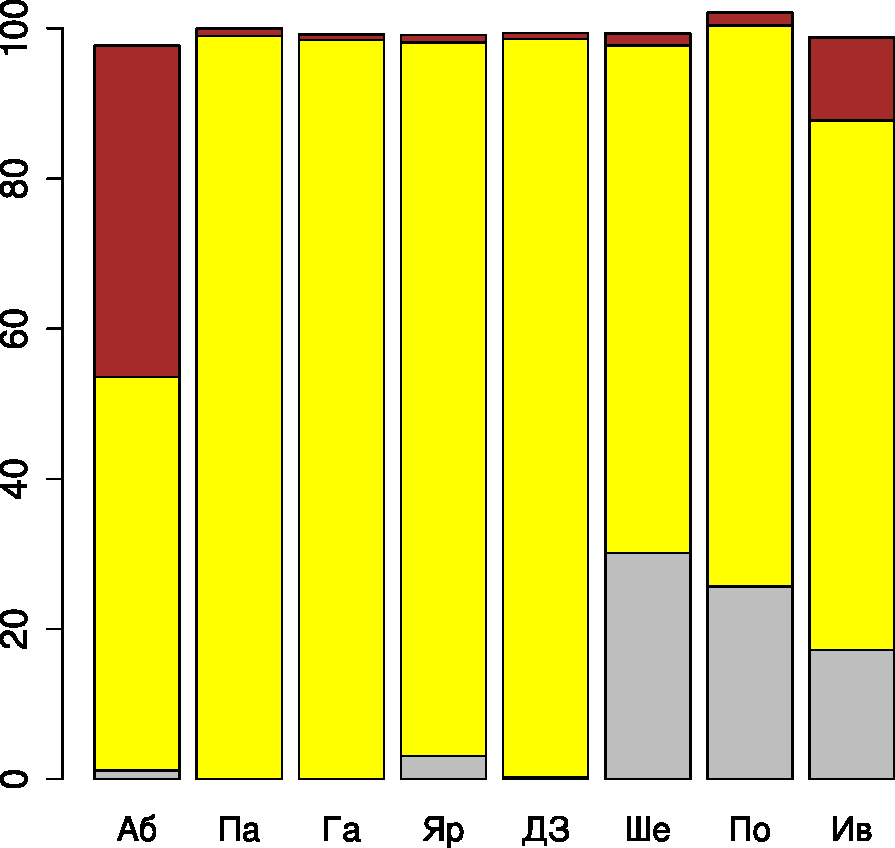
\includegraphics[width=\textwidth]{grunty_barents1.pdf}
%		\end{center}
%	\end{minipage}

%\begin{tiny} 
%Обозначения участков: ЗРС~--- Западная Ряшкова Салма, Аб~--- Абрам-мыс, Па~--- Пала-губа, Га~--- Гаврилово, Яр~--- Ярнышная, ДЗ~--- Дальне-Зеленецкая, Ше~--- Шельпино, По~--- Порчниха, Ив~--- Ивановская.\\
%\end{tiny}
%{\scriptsize Цветовые обозначения: серый~--- гравий, желтый~--- песок, коричневый~--- алевриты и пелиты.}
{\tiny Цветовые обозначения районов: Красный~--- Керетский архипелаг, синий~--- Северный архипелаг, зеленый~--- Лувеньгские шхеры, голубой~--- Кольский залив, фиолетовый~--- Восточный Мурман}
\end{frame}

\begin{frame}{Совокупное таксономическое разнообразие в сообщестах}
		\begin{flushleft}
		\textcolor{blue}{\footnotesize Белое море (57 таксонов)}\\
			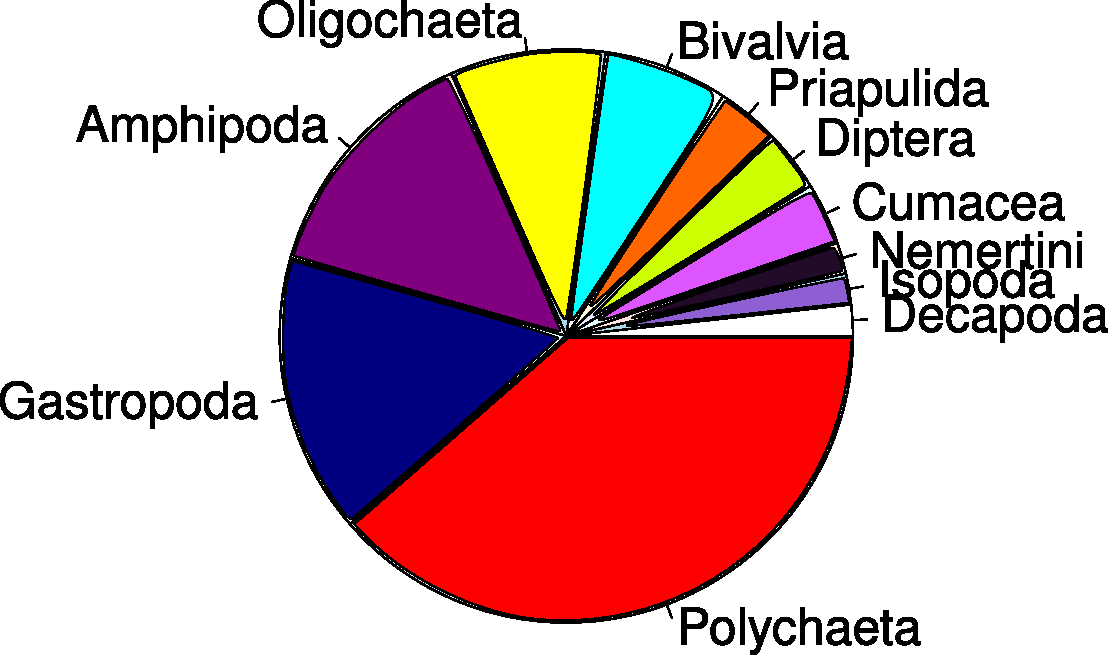
\includegraphics[height=0.34\textheight]{White_taxons_pie_big1.pdf}
		\end{flushleft}

		\begin{flushright}
		\textcolor{blue}{\footnotesize Баренцево море (48 таксонов)}\\
			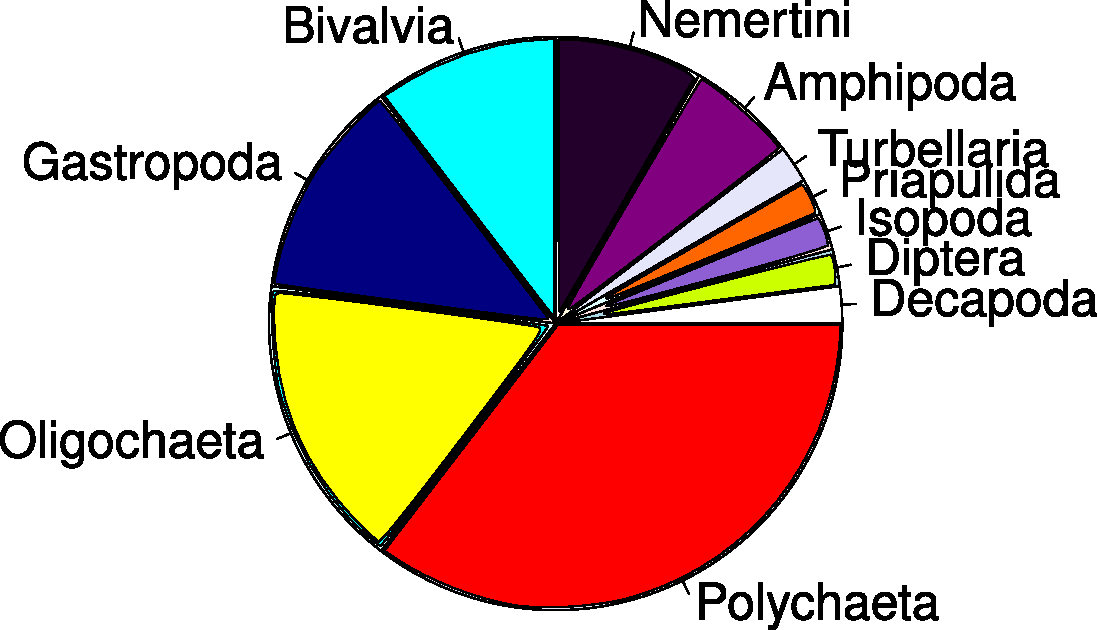
\includegraphics[height=0.34\textheight]{Barents_taxons_pie_big1.pdf}
		\end{flushright}
\end{frame}


%%%%%%%%%%%%%%%%%%%%%%%%%%%%%%%%%%%%%%%%%%%%%%%%%%%%%
		\section[Обилие]{Обилие {\it Macoma balthica}}
%%%%%%%%%%%%%%%%%%%%%%%%%%%%%%%%%%%%%%%%%%%%%%%%%%%%%
\begin{frame}{Обилие {\it M.~balthica} в Белом море}
	\begin{minipage}[t]{.49\linewidth}
		\begin{center}
		{\footnotesize Плотность поселения}
			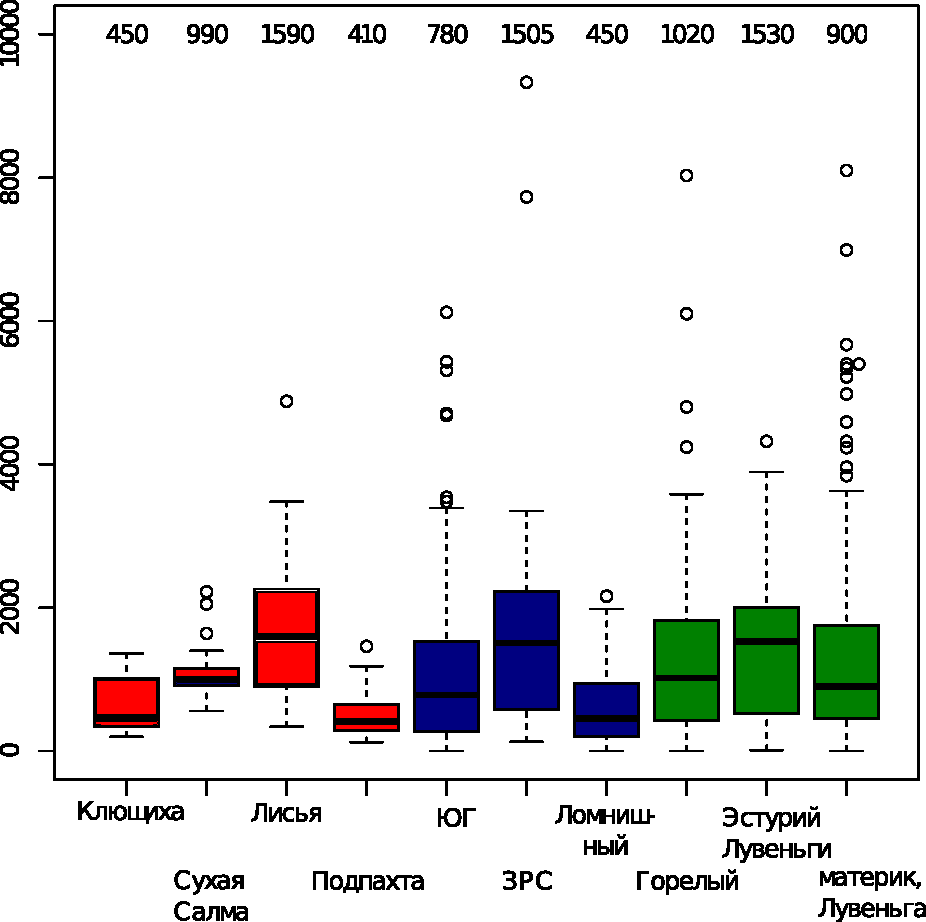
\includegraphics[width=\textwidth]{N2_area_White2.pdf}
		\end{center}
	\end{minipage}
%
	\begin{minipage}[t]{.49\linewidth}
		\begin{center}
		{\footnotesize Биомасса}
			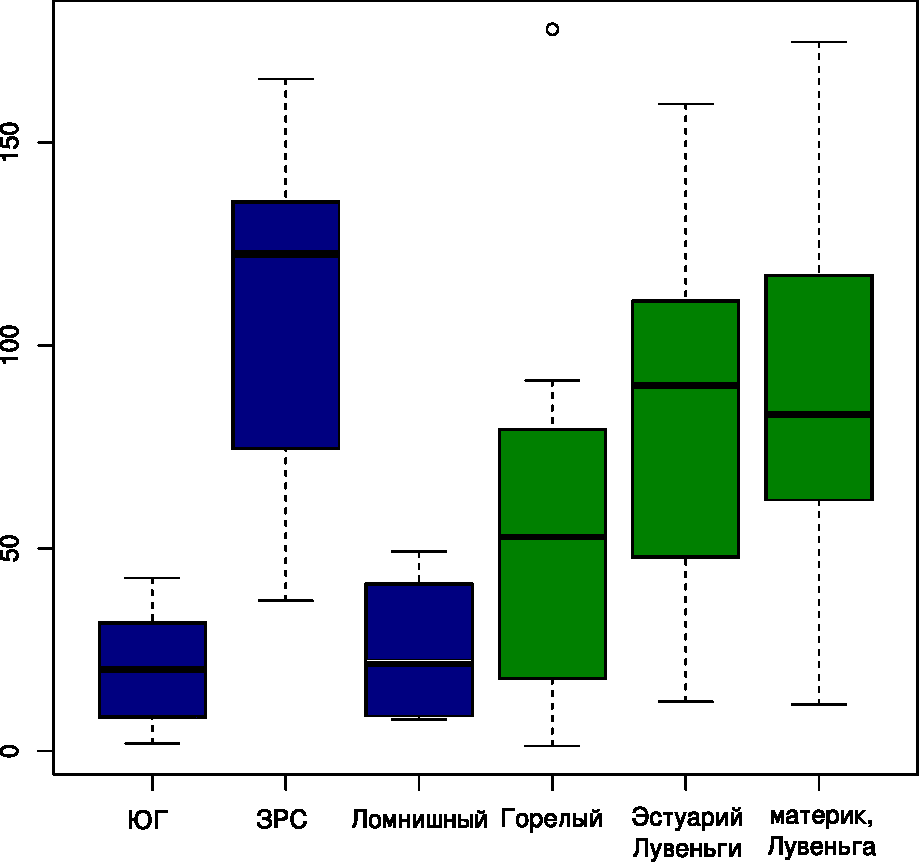
\includegraphics[width=\textwidth]{B_Kanda_ru2.pdf}
		\end{center}
	\end{minipage}


{\scriptsize Районы: Керетский архипелаг~--- красный, Северный архипелаг~--- синий, Лувеньгские шхеры~--- зеленый.}\\[1ex]
\begin{tiny} 
Жирная горизонтальная линия~--- медианное значение показателя;\\
границы <<ящика>>~--- 1 и 3 квартили;\\ <<усы>>~--- 1,5 интерквартильного расстояния;\\ 
точки~--- значения, выпадающие за 1,5 интерквартильных расстояния.\\ 
Числа в верхней части графика~--- средние значения плотности поселений маком, экз./м$^2$.
\end{tiny}

\end{frame}



\begin{frame}{Обилие {\it M.~balthica} в Баренцевом море}
	\begin{minipage}[t]{.49\linewidth}
		\begin{center}
		{\footnotesize Плотность поселения}
			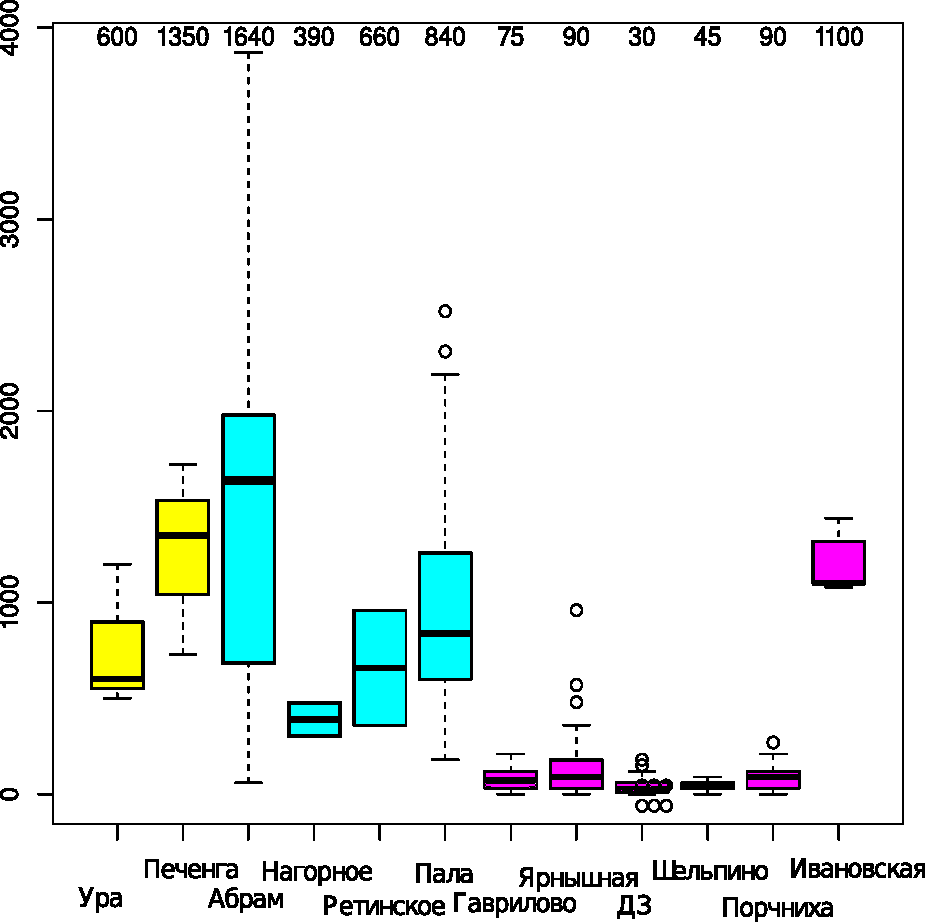
\includegraphics[width=\textwidth]{N2_area_Barents2.pdf}
		\end{center}
	\end{minipage}
%
	\begin{minipage}[t]{.49\linewidth}
		\begin{center}
		{\footnotesize Биомасса}
			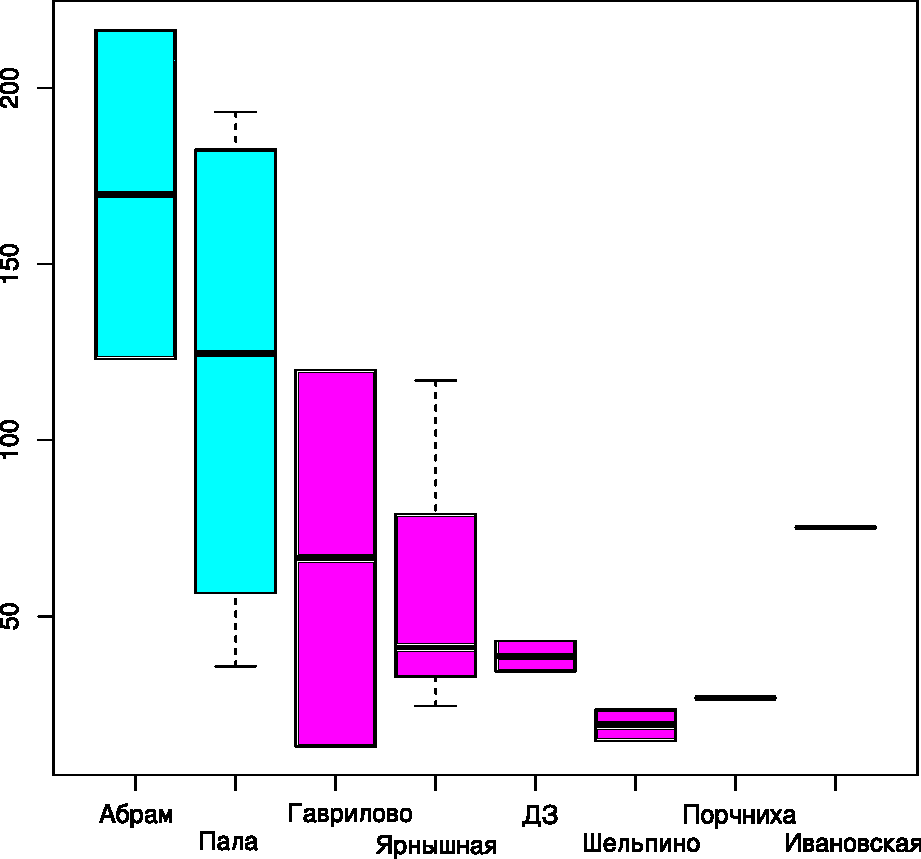
\includegraphics[width=\textwidth]{B_Barents_uchastki_ru2.pdf}
		\end{center}
	\end{minipage}


{\scriptsize Районы: Западный Мурман ~--- желтый, Кольский залив~--- голубой, Восточный Мурман~--- фиолетовый.}\\[1ex]
\begin{tiny}
 Жирная горизонтальная линия~--- медианное значение показателя;\\
границы <<ящика>>~--- 1 и 3 квартили;\\ <<усы>>~--- 1,5 интерквартильного расстояния;\\ 
точки~--- значения, выпадающие за 1,5 интерквартильных расстояния.\\ 
Числа в верхней части графика~--- средние значения плотности поселений маком, экз./м$^2$.
\end{tiny}
\end{frame}



\begin{frame}{Обилие {\it M.~balthica} в европейской части ареала}
	\begin{minipage}[t]{.49\linewidth}
		\begin{center}
		{\footnotesize Плотность поселения}
			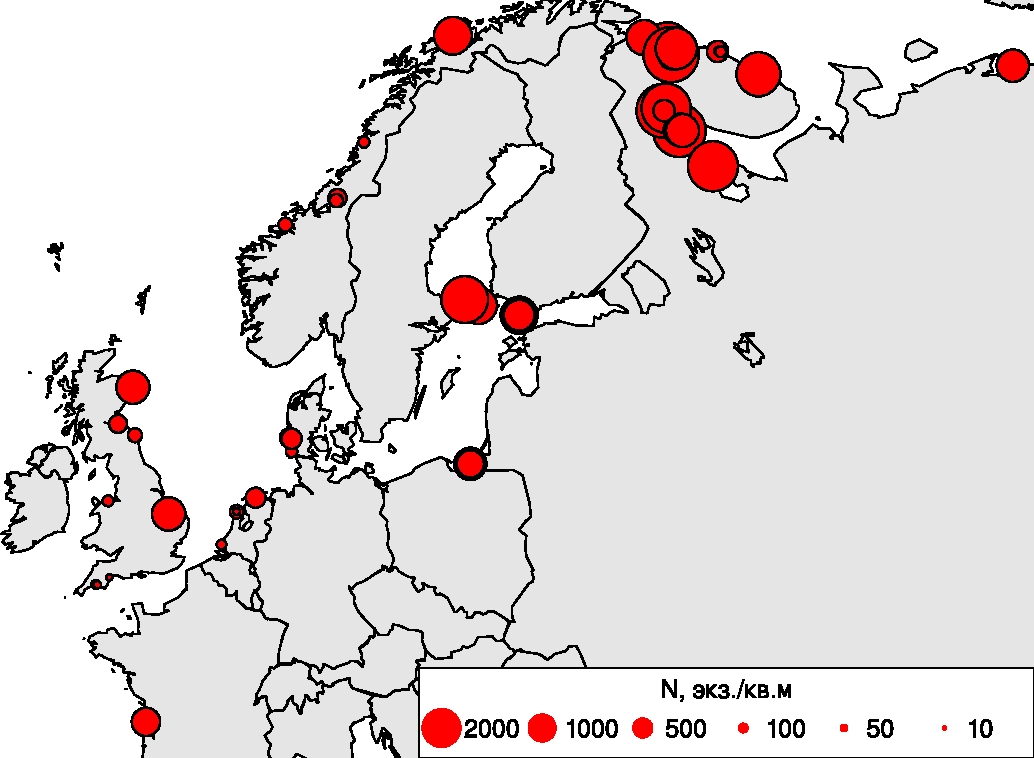
\includegraphics[width=\textwidth]{Nmean_ru1.pdf}\\[1ex]
			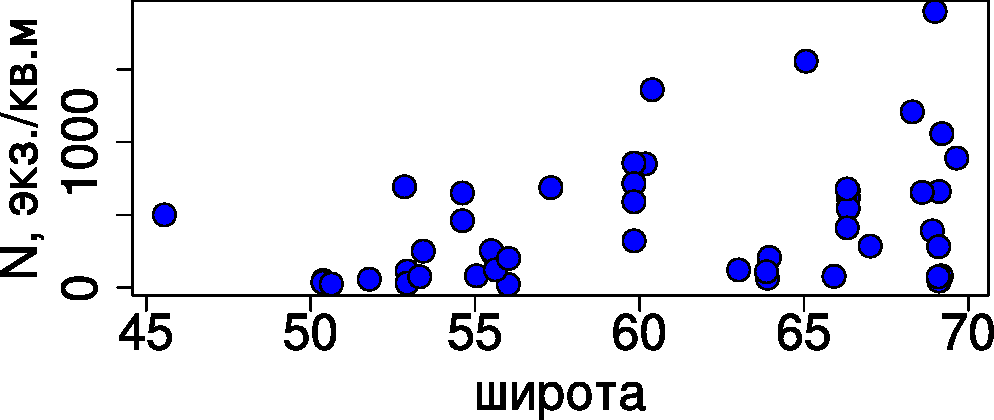
\includegraphics[width=\textwidth]{lat_vs_Nmean_big1.pdf}\\
{\small Корреляция Спирмена: $r_{s} = -0,43$, $p < 0,0006$.}
		\end{center}
	\end{minipage}
%
	\begin{minipage}[t]{.49\linewidth}
		\begin{center}
		{\footnotesize Биомасса}
			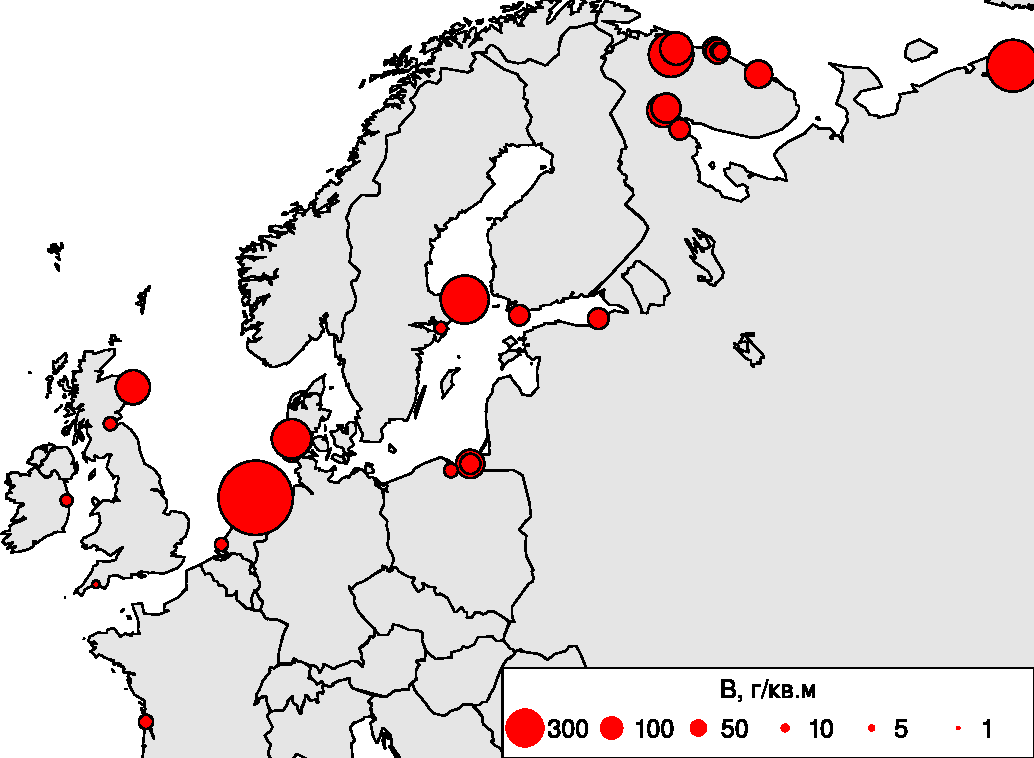
\includegraphics[width=\textwidth]{Bmean_ru1.pdf}\\[1ex]
			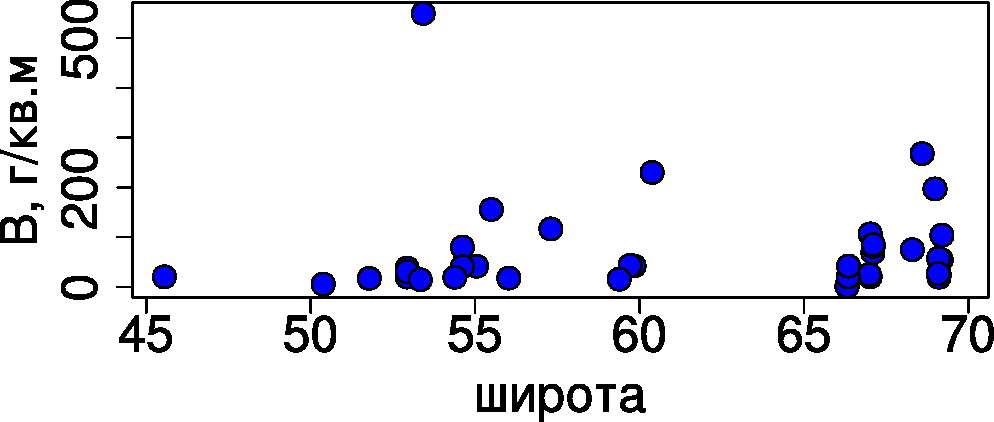
\includegraphics[width=\textwidth]{lat_vs_Bmean_big1.pdf}\\
{\small Корреляция Спирмена: $r_{s} = -0,3$, $p < 0,06$.}
		\end{center}
	\end{minipage}

{\tiny Средние значения показателей пропорциональны площади круга на карте}
\end{frame}



%%%%%%%%%%%%%%%%%%%%%%%%%%%%%%%%%%%%%%%%%%%%%%%%%%%%%
		\section[Динамика численности]{Динамика плотности поселений {\it Macoma balthica} в Белом море}
%%%%%%%%%%%%%%%%%%%%%%%%%%%%%%%%%%%%%%%%%%%%%%%%%%%%%
\begin{frame}{Динамика плотности поселений {\it M.~balthica} в вершине Кандалакшского залива}
	\begin{minipage}[t]{.49\linewidth}
		\begin{center}
			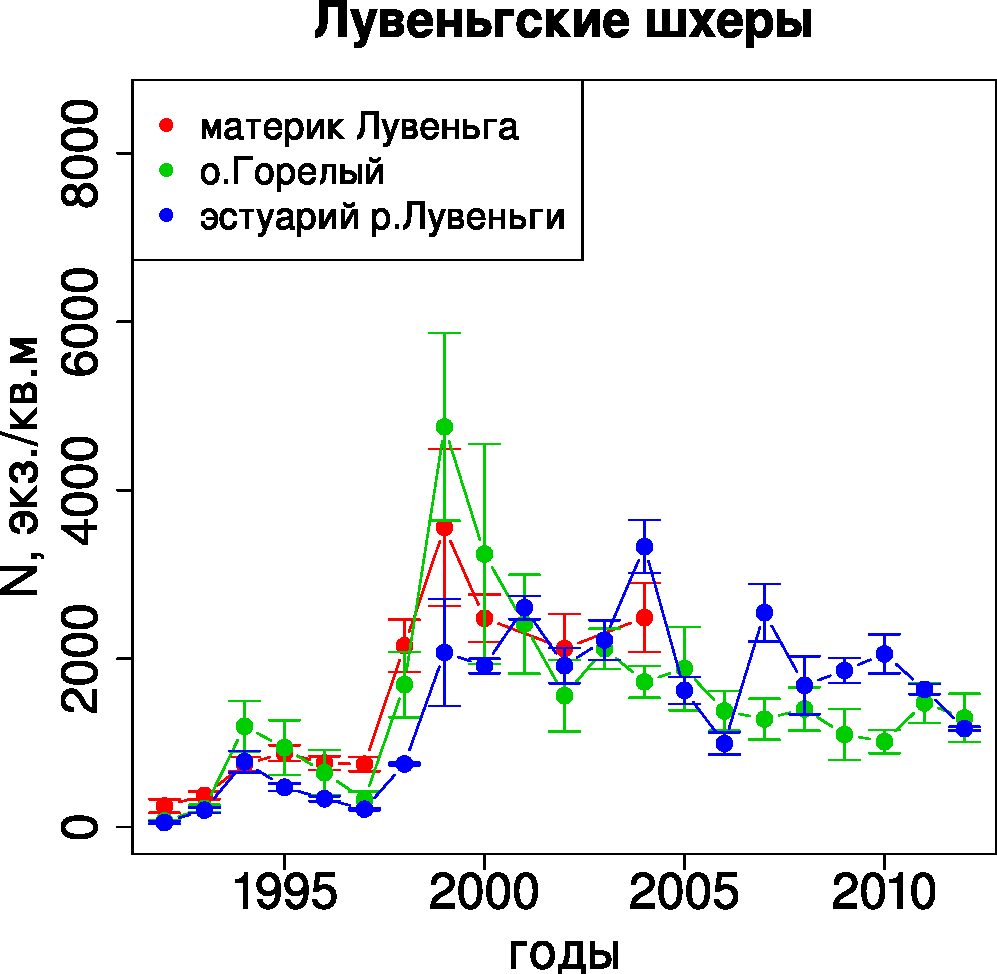
\includegraphics[width=\textwidth]{N2_dynamic_Luvenga_big1.pdf}
		\end{center}
	\end{minipage}
%
	\begin{minipage}[t]{.49\linewidth}
		\begin{center}
			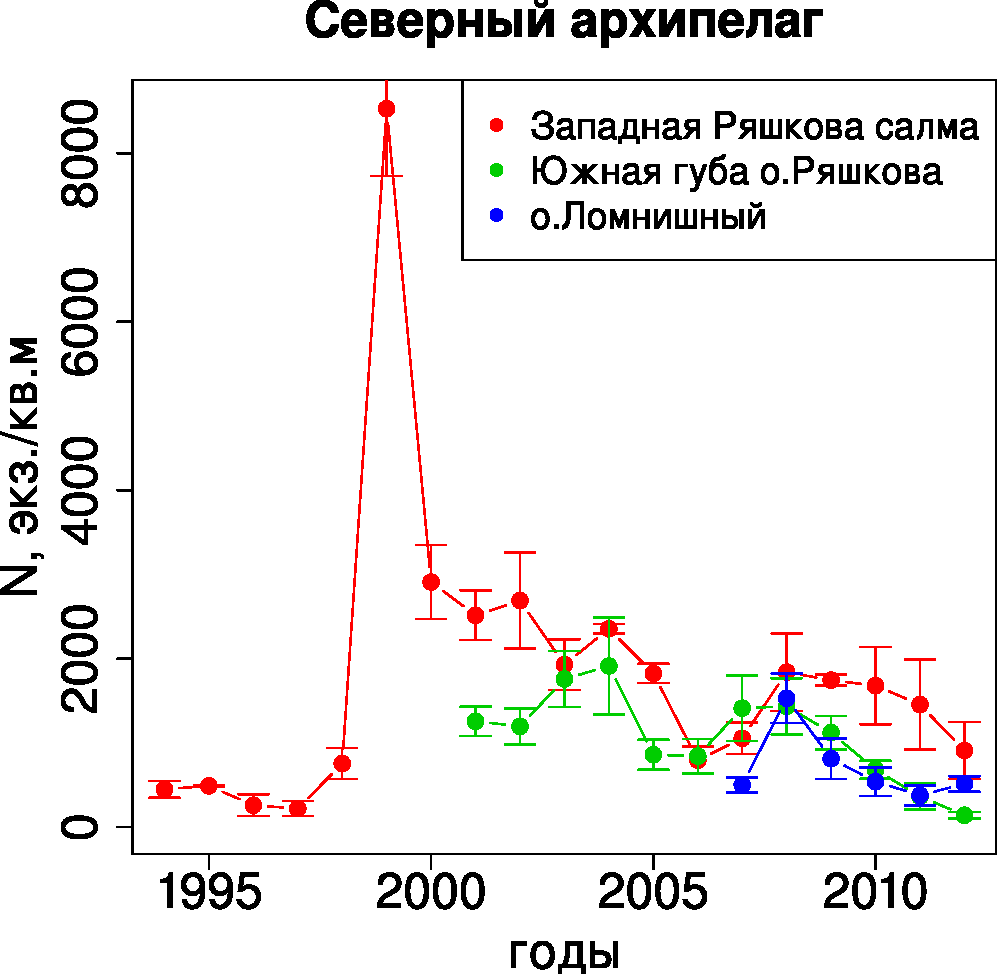
\includegraphics[width=\textwidth]{N2_dynamic_North_big1.pdf}
		\end{center}
	\end{minipage}
{\tiny По оси ординат указана средняя плотность поселения без учета спата}
\end{frame}

\begin{frame}{Синхронность динамики плотности поселений {\it M.~balthica} в Кандалакшском заливе Белого моря}
		\begin{center}
%			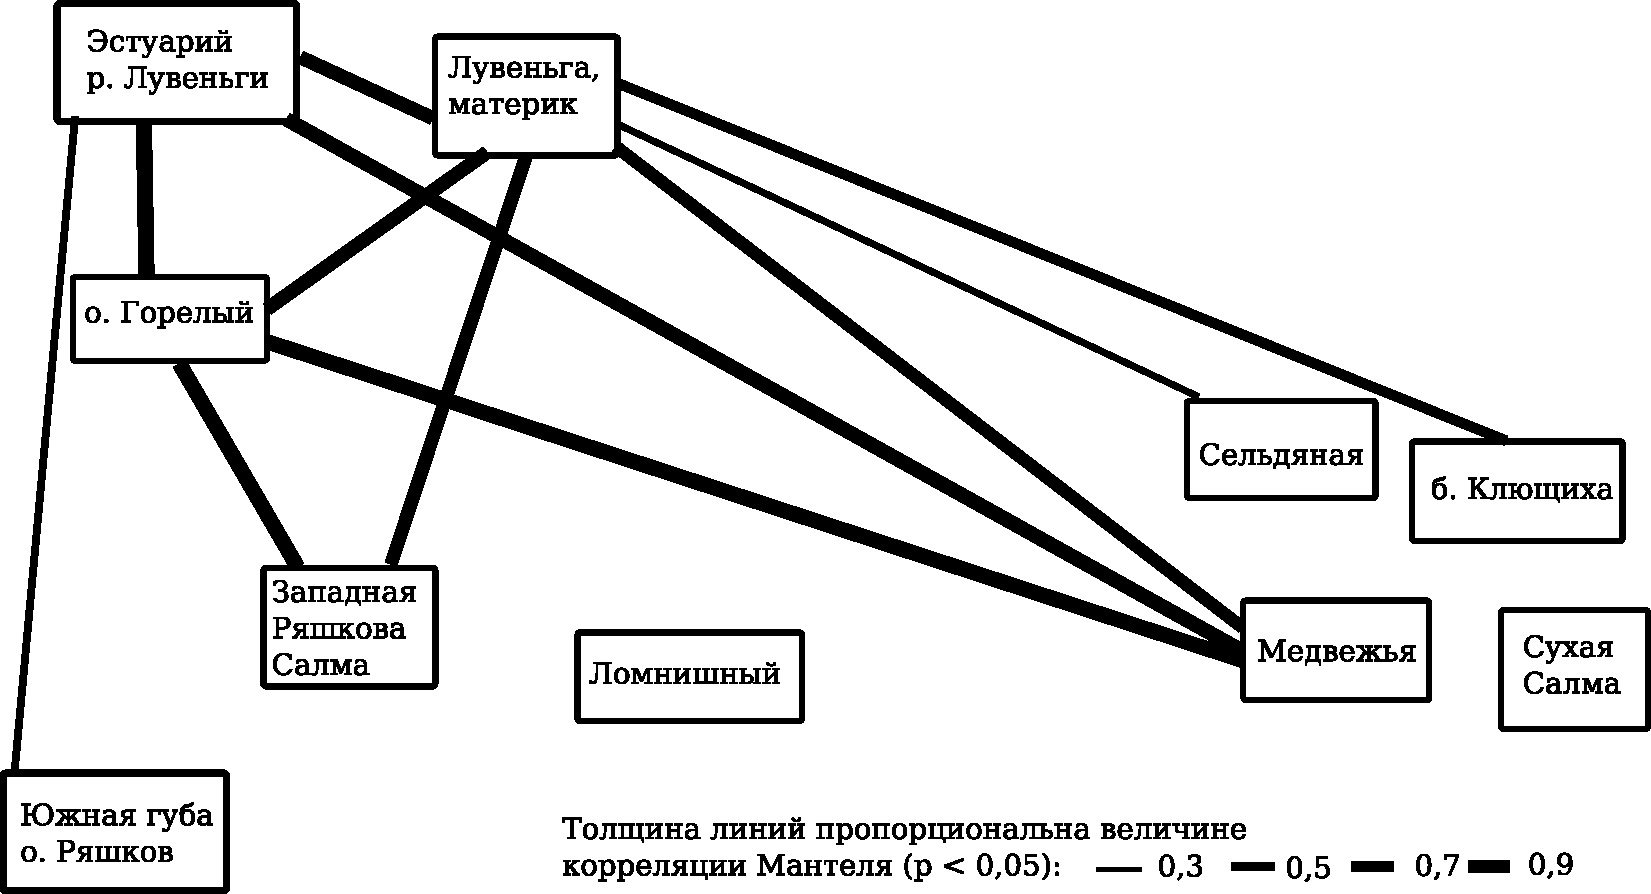
\includegraphics[width=\textwidth]{mantel1.pdf}
			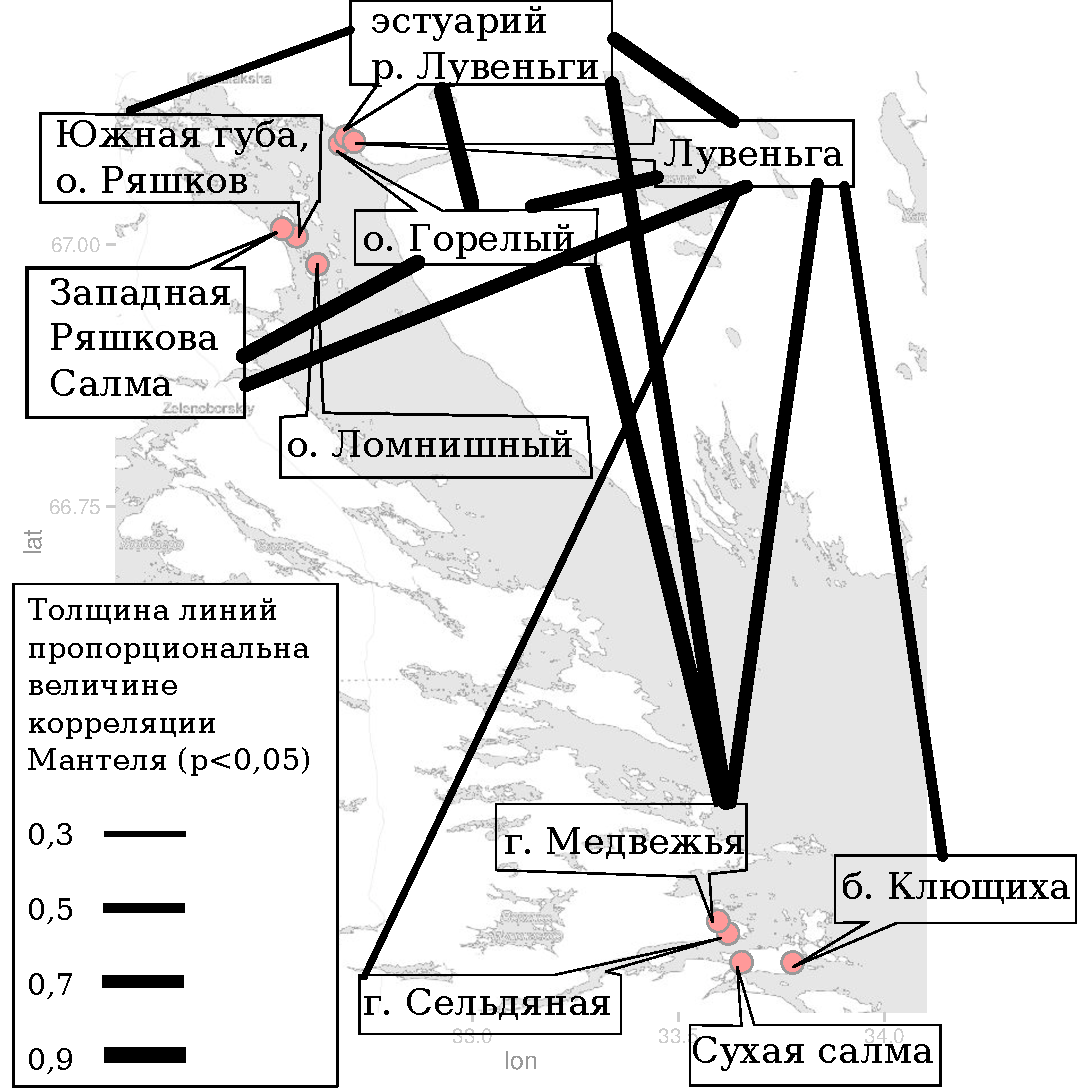
\includegraphics[height=.7\textheight]{mantel_map.pdf}
		\end{center}
\end{frame}


\begin{frame}{Моделирование влияния температуры на численность {\it M.~balthica} в Кандалакшском заливе Белого моря}
$$\ln(N_{t1}) = 1,96 + 0,60 \times \ln(N_{t}) - 0,09 \times T_{wt1}$$
{\scriptsize $F = 37,04$; $p < 0,0001$. $R^2 = 0,6$.} \\
	\begin{minipage}[t]{.49\linewidth}
		\begin{center}
			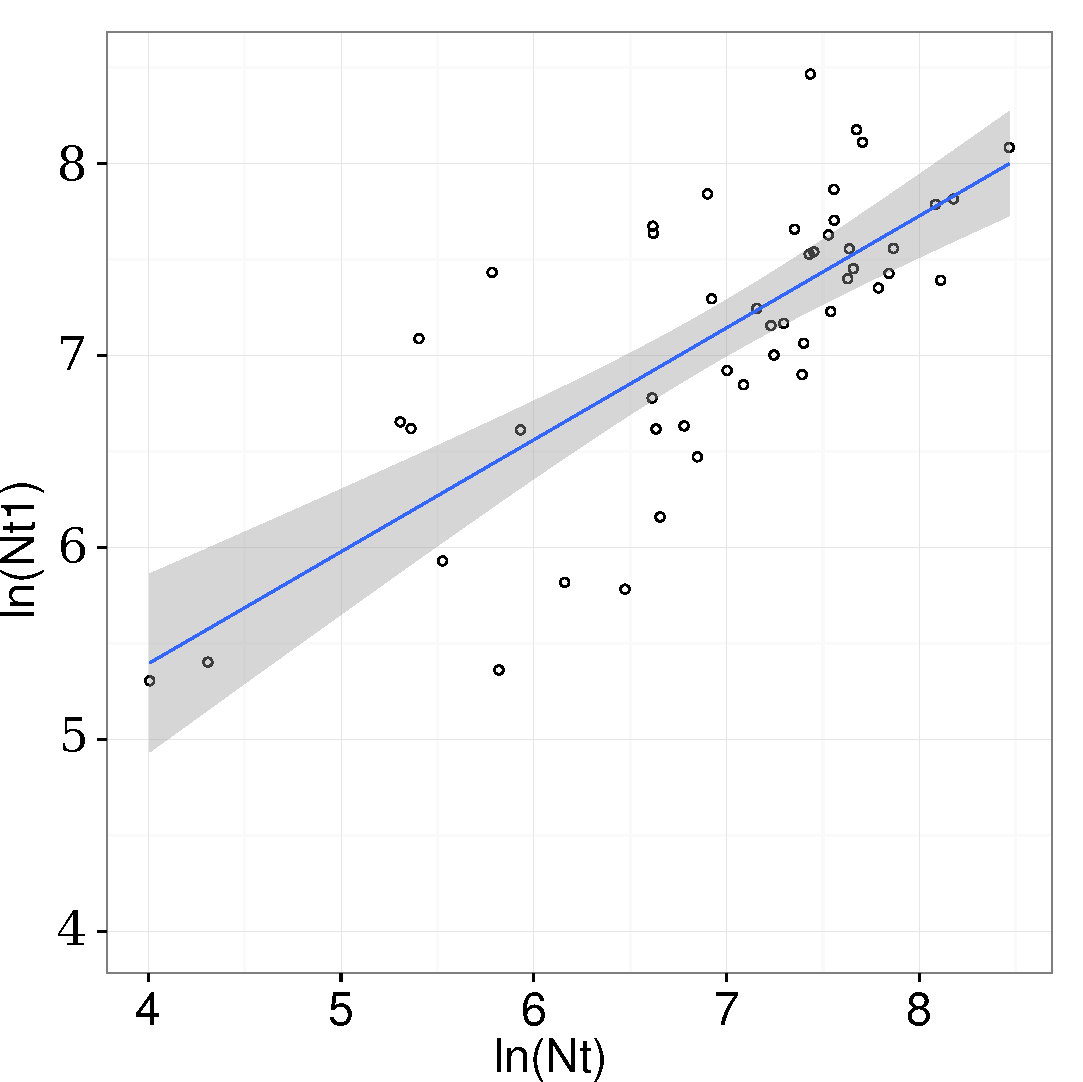
\includegraphics[width=\textwidth]{./lodNt_vs_logNt1_2.pdf}
		\end{center}
	\end{minipage}
%
	\begin{minipage}[t]{.49\linewidth}
		\begin{center}
			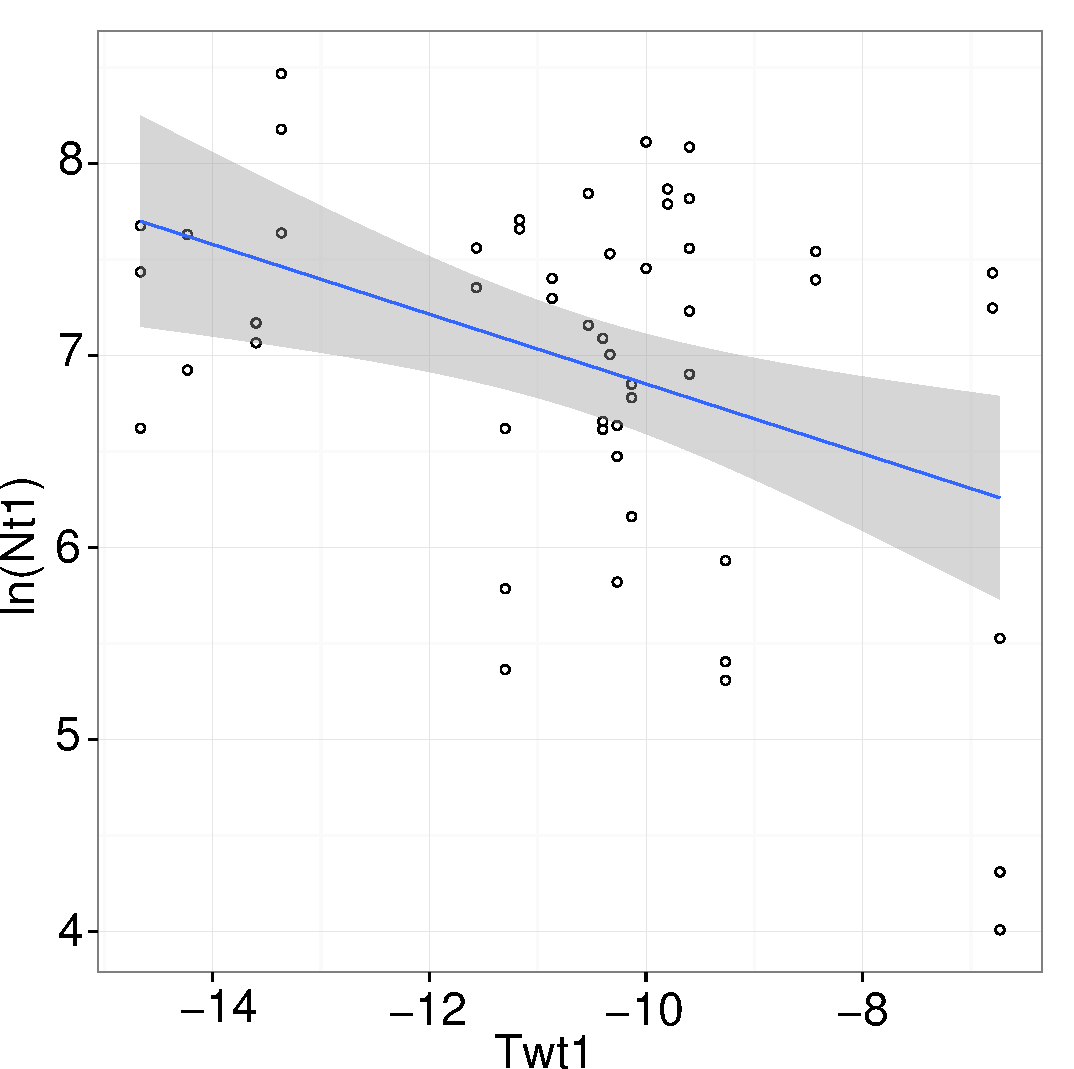
\includegraphics[width=\textwidth]{./Twt1_vs_logNt1_2.pdf}
		\end{center}
	\end{minipage}
{\tiny $\log(N_{t1})$ и $\log(N_{t})$~--- логарифм средней численности маком в данный ($t1$) и предыдущий ($t$) годы; $T_{wt1}$~--- среднезимняя температура в текущий год.}
\end{frame}

%%%%%%%%%%%%%%%%%%%%%%%%%%%%%%%%%%%%%%%%%%%%%%%%%%%%%
		\section[Размерная структура]{Характер размерной структуры поселений {\it Macoma balthica}}
%%%%%%%%%%%%%%%%%%%%%%%%%%%%%%%%%%%%%%%%%%%%%%%%%%%%%

\begin{frame}{Характерные варианты размерно-частотного распределения особей {\it M.~balthica} в поселениях}
	\begin{minipage}[t]{.48\linewidth}
		\begin{center}
{\footnotesize Белое море}\\
			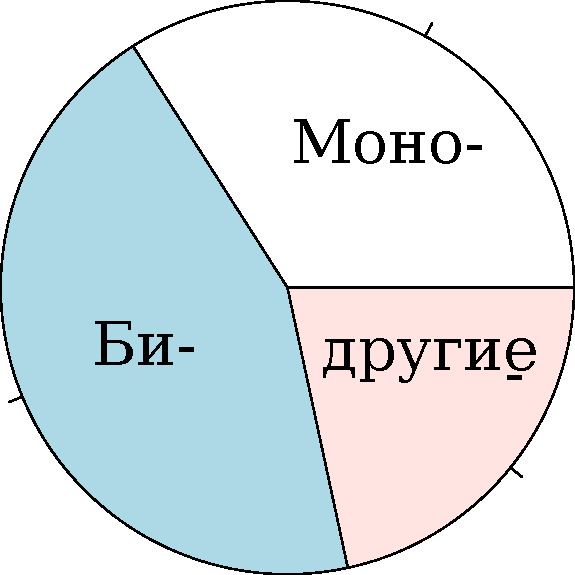
\includegraphics[height=.2\textheight]{White_freq_types.pdf}
		\end{center}
	\end{minipage}
%
	\begin{minipage}[t]{.48\linewidth}
		\begin{center}
{\footnotesize Баренцево море}\\
			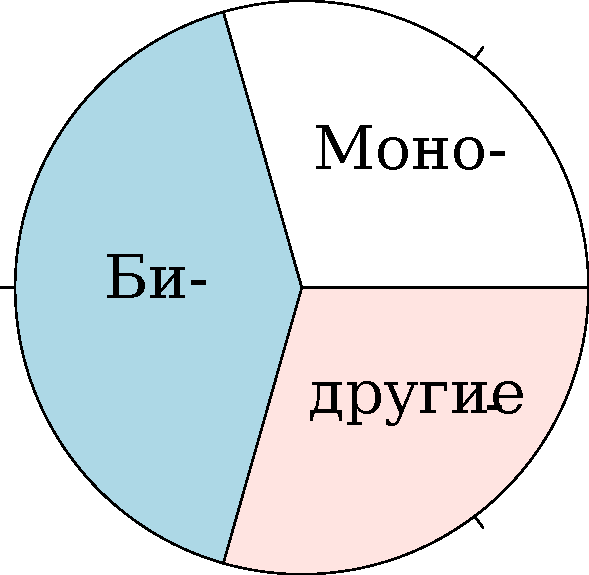
\includegraphics[height=.2\textheight]{Barents_freq_types.pdf}
		\end{center}
	\end{minipage}

\hrulefill

	\begin{tabularx}{\linewidth}{XX|XX}
		\multicolumn{2}{c|}{\footnotesize Бимодальное} & \multicolumn{2}{c}{\footnotesize Мономодальное} \\
			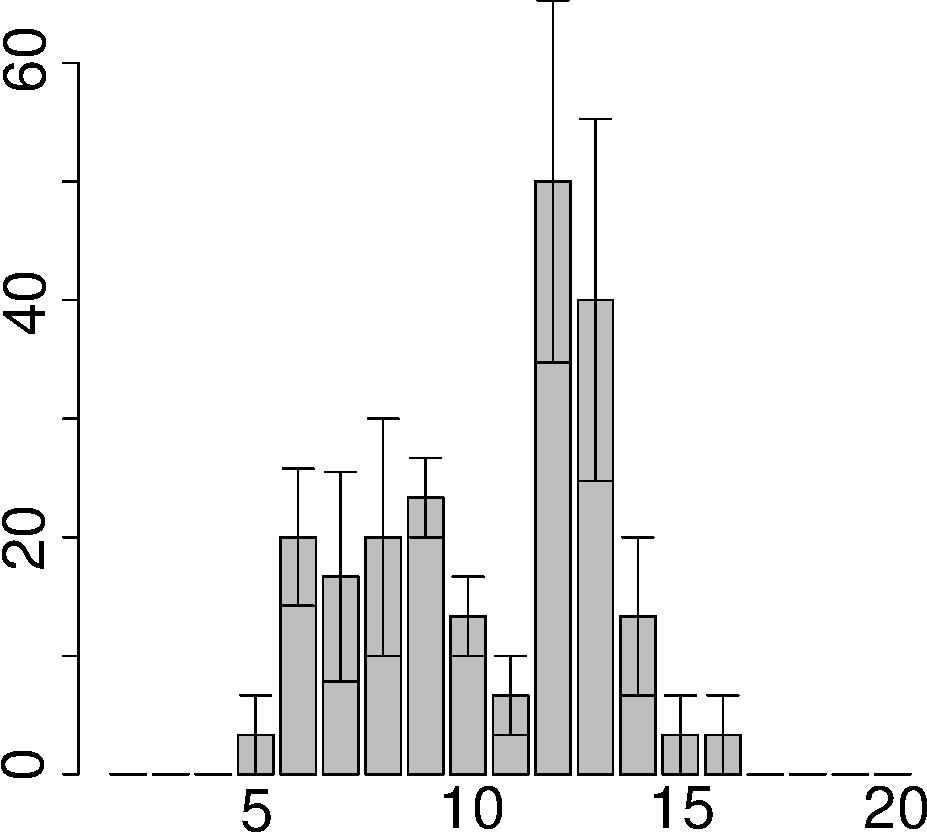
\includegraphics[width=\linewidth]{sizestr2_1997_.pdf} & 
			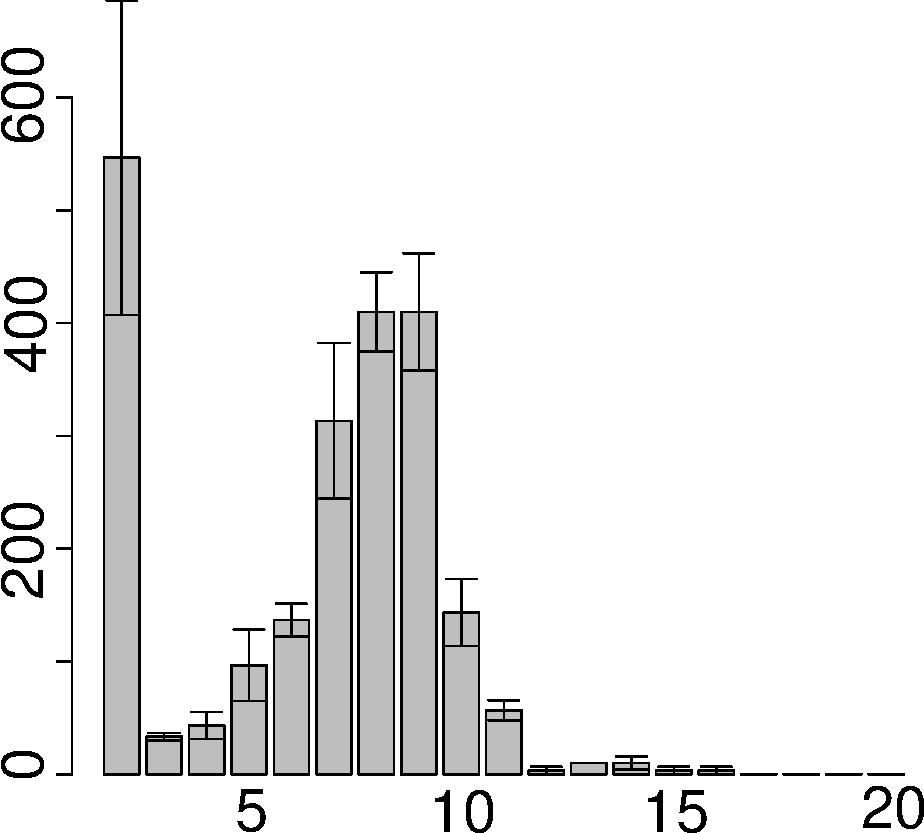
\includegraphics[width=\linewidth]{sizestr2_2003_.pdf} & 
			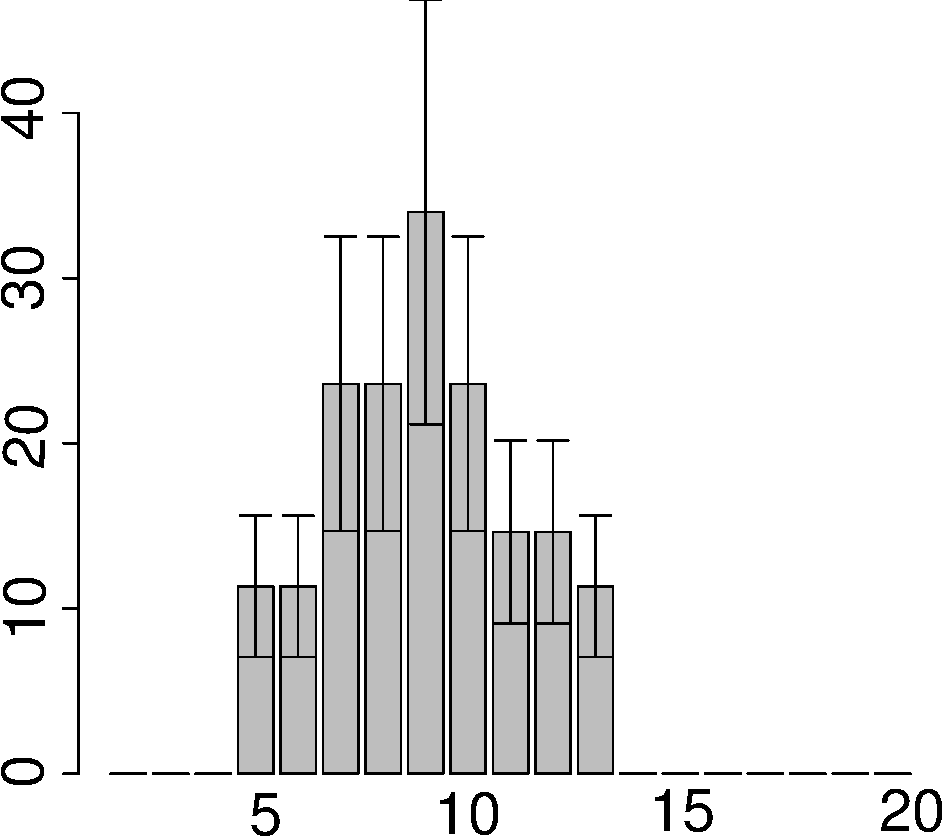
\includegraphics[width=\linewidth]{high_beatch2_1992_.pdf} &
			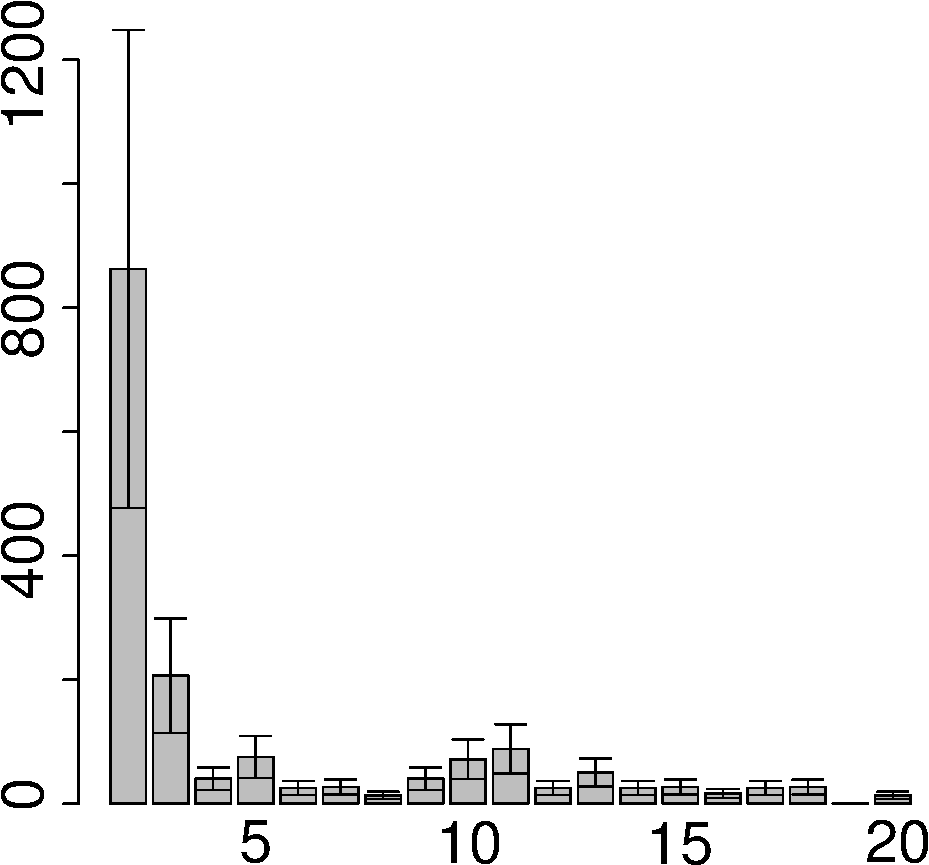
\includegraphics[width=\linewidth]{zostera_zone2_1998_.pdf}  \\
			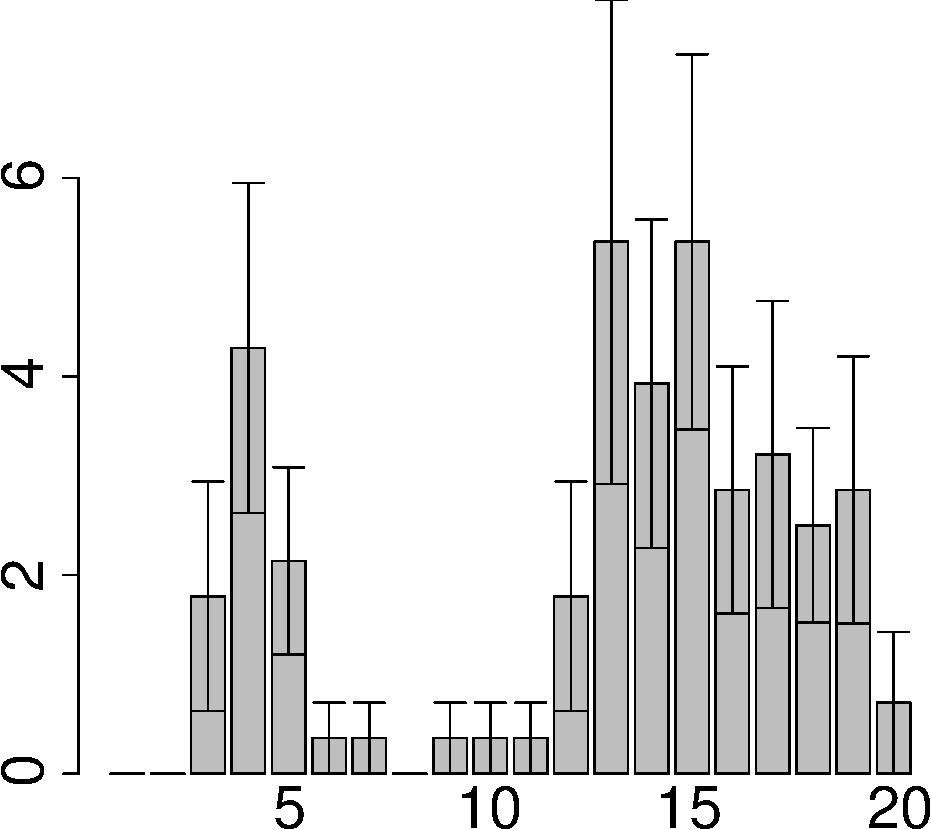
\includegraphics[width=\linewidth]{DZ_2006_.pdf} & 
			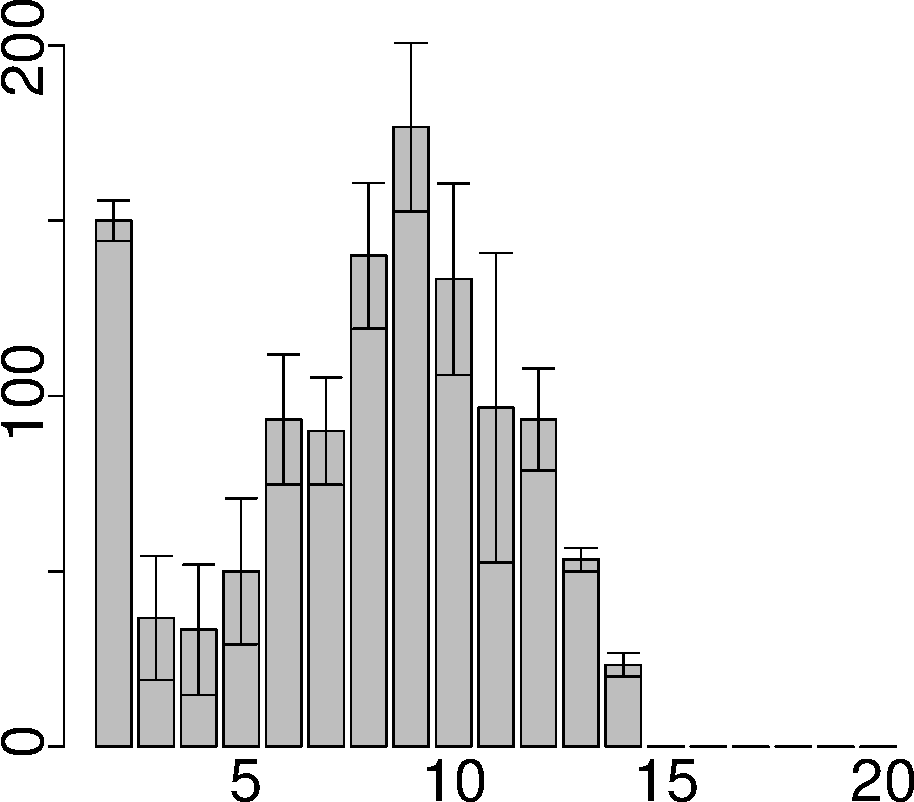
\includegraphics[width=\linewidth]{sizestr2_2012_.pdf} & 
			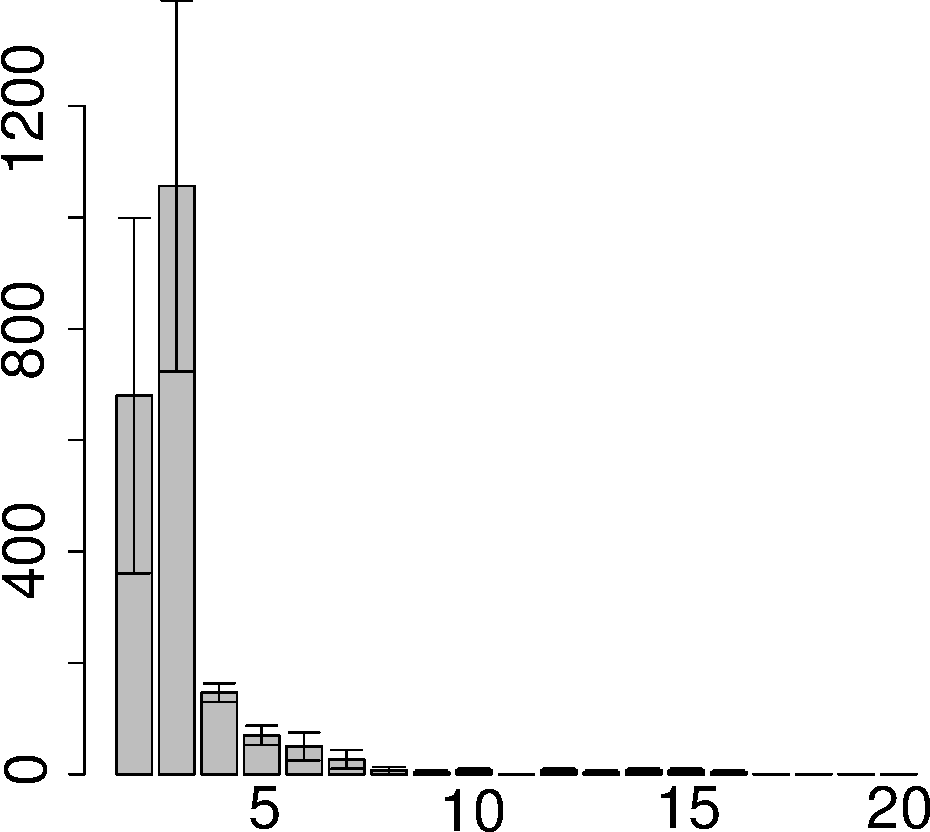
\includegraphics[width=\linewidth]{sizestr2_1999_.pdf} &
			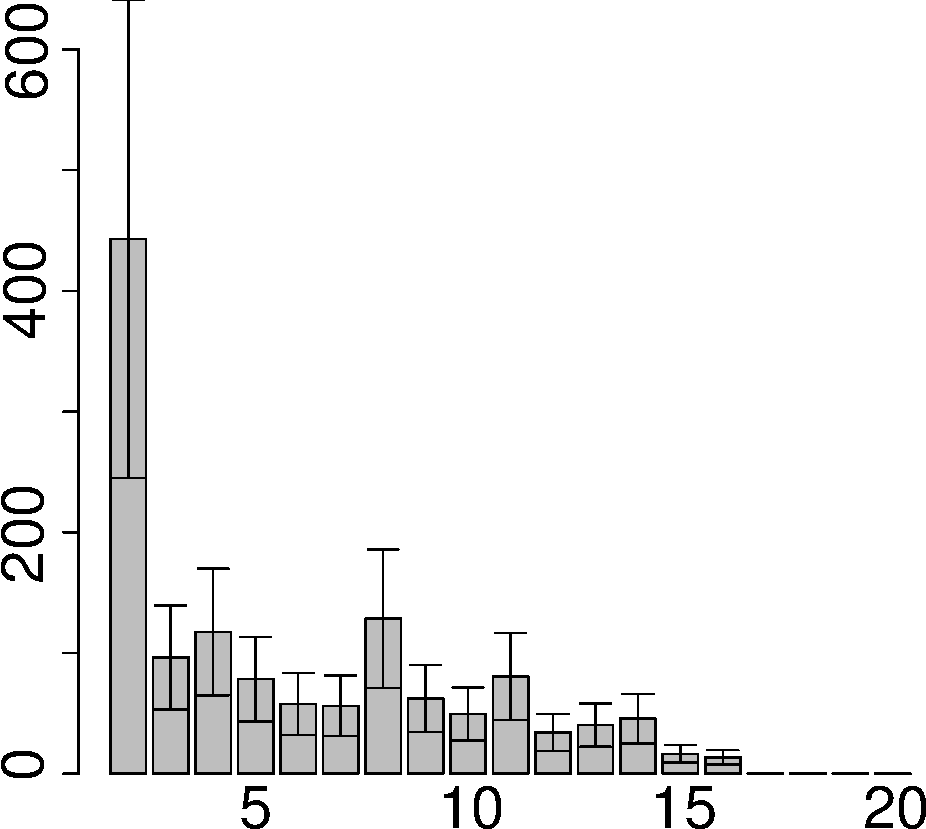
\includegraphics[width=\linewidth]{zostera_zone2_2004_.pdf}  \\
\end{tabularx}
{\tiny Абсцисса~--- длина раковины, мм; ордината~--- численность, экз./м$^2$.}
\end{frame}


\begin{frame}{Динамика размерной структуры: чередование вариантов распределения}
Пример: эстуарий р.~Лувеньги\\[2ex]

			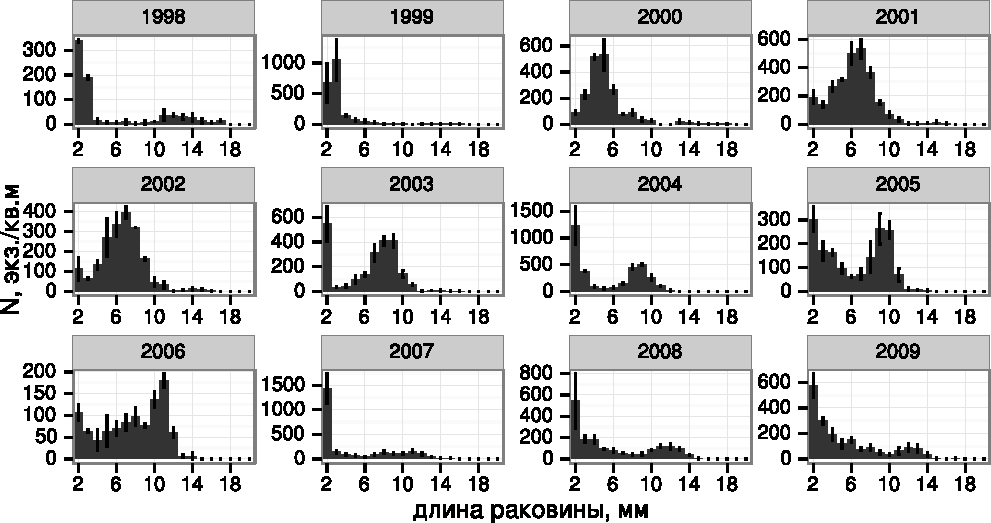
\includegraphics[width=\textwidth]{Estuary_total_size_oneplot_nonscale1.pdf}\\
\end{frame}



\begin{frame}{Динамика размерной структуры: повторение мономодального распределения}
Пример: Южная губа острова Ряшкова\\[2ex]

			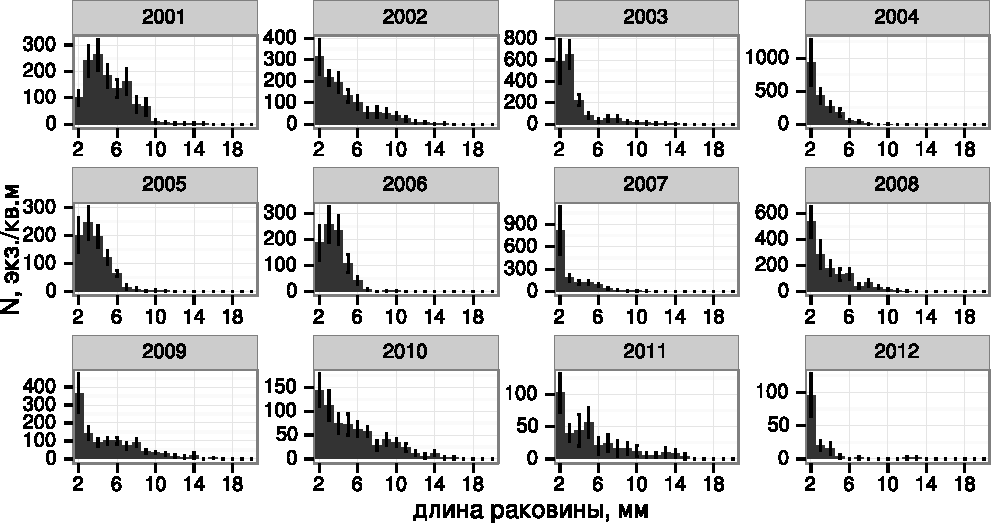
\includegraphics[width=\textwidth]{YuG_sizestr_oneplot_nonscale1.pdf}
\end{frame}



\begin{frame}{Организация поселений {\it M.~balthica}: динамика размерной структуры}
	\begin{minipage}[t]{.53\linewidth}
		\begin{center}
			{\scriptsize Распространение типов динамики размерной структуры в Белом море}\\
			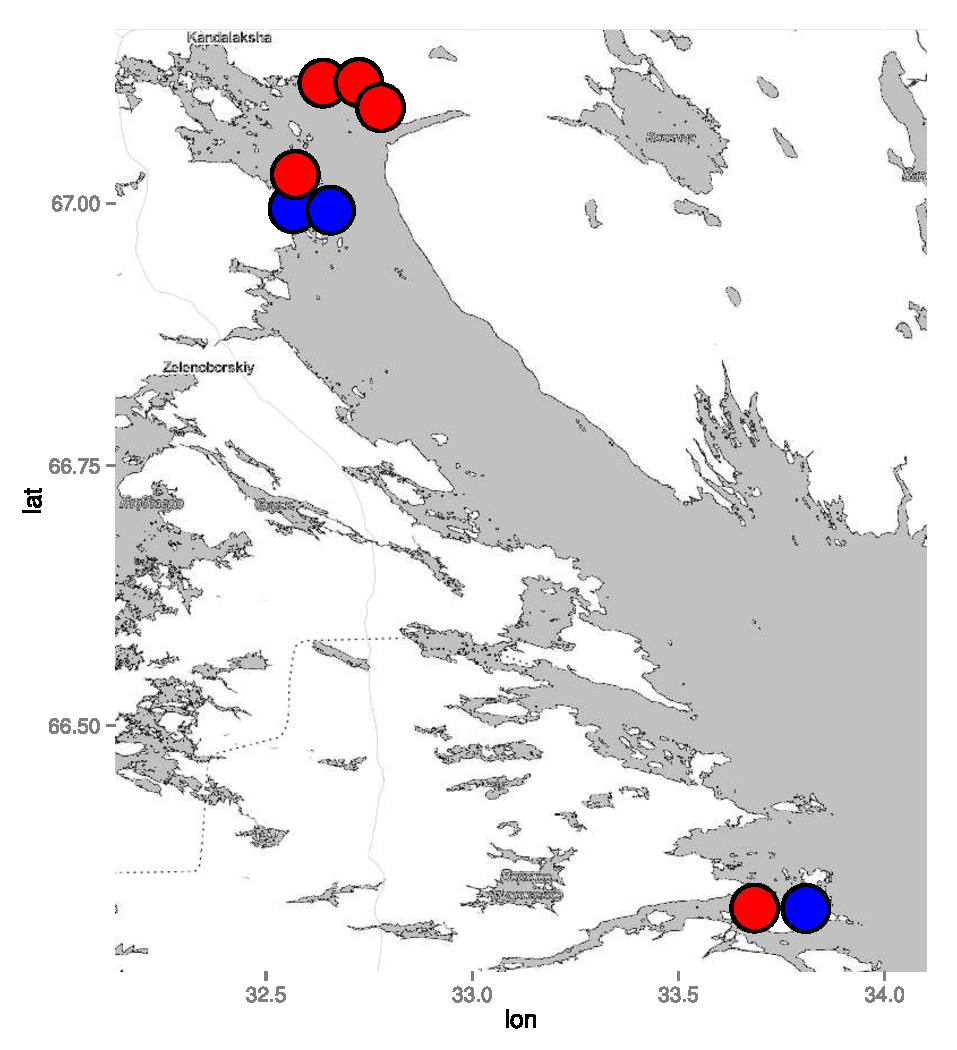
\includegraphics[width=\textwidth]{map_size_distr.pdf}\\
\textcolor{red}{\scriptsize +поселение в г.~Дальне-Зенеленцкой Баренцева моря}
		\end{center}

	\end{minipage}
%
	\begin{minipage}[t]{.45\linewidth}
		\begin{center}
	\textcolor{red}{\footnotesize Чередование вариантов\\ размерной структуры}
			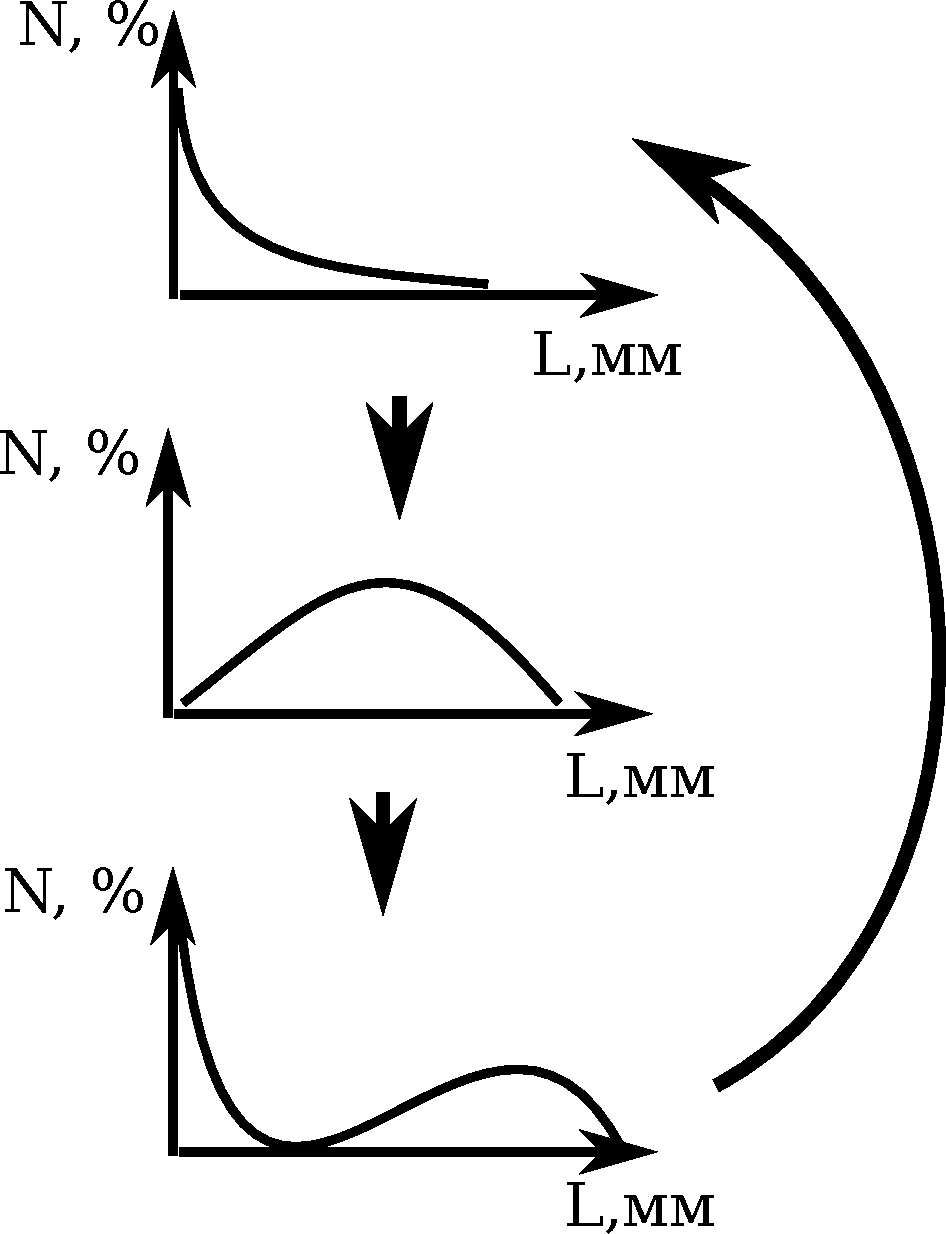
\includegraphics[width=.65\textwidth]{Dymanic_cheredovanie.pdf}

	\textcolor{blue}{\footnotesize Ежегодное повторение\\ размерной структуры}\\
			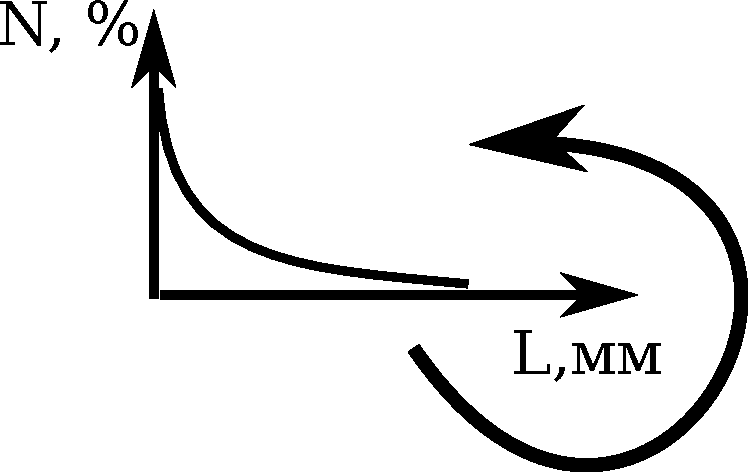
\includegraphics[width=.65\textwidth]{Dymanic_povtorenie.pdf}\\


		\end{center}
	\end{minipage}
\end{frame}

%%%%%%%%%%%%%%%%%%%%%%%%%%%%%%%%%%%%%%%%%%%%%%%%%%%%%
		\section[Линейный рост]{Линейный рост {\it Macoma balthica}}
%%%%%%%%%%%%%%%%%%%%%%%%%%%%%%%%%%%%%%%%%%%%%%%%%%%%%
\begin{frame}{Линейный рост {\it M.~balthica} в Баренцевом море}
	\begin{minipage}[t]{.58\linewidth}
		\begin{center}
			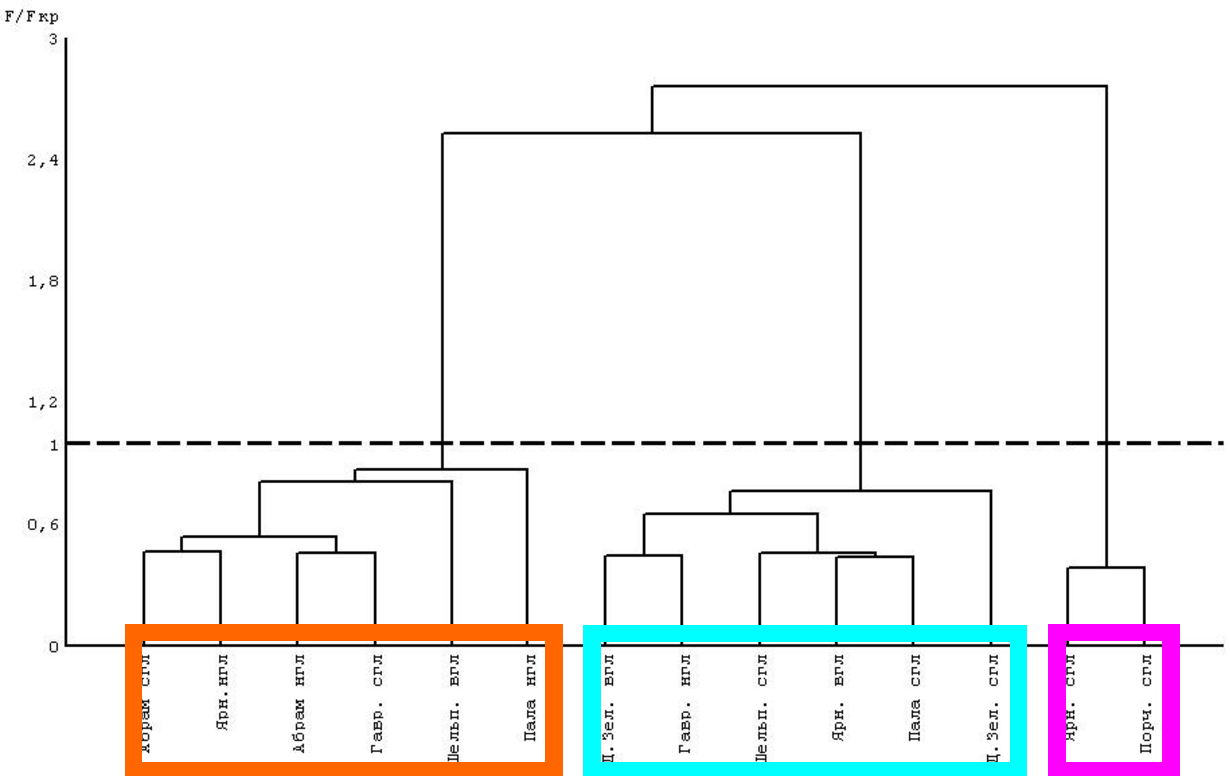
\includegraphics[width=\textwidth]{./dendrogramma_sravnenie_rosta_linear_all_gorizonts.pdf}
		\end{center}
	\end{minipage}
%
	\begin{minipage}[t]{.4\linewidth}
		\begin{center}
			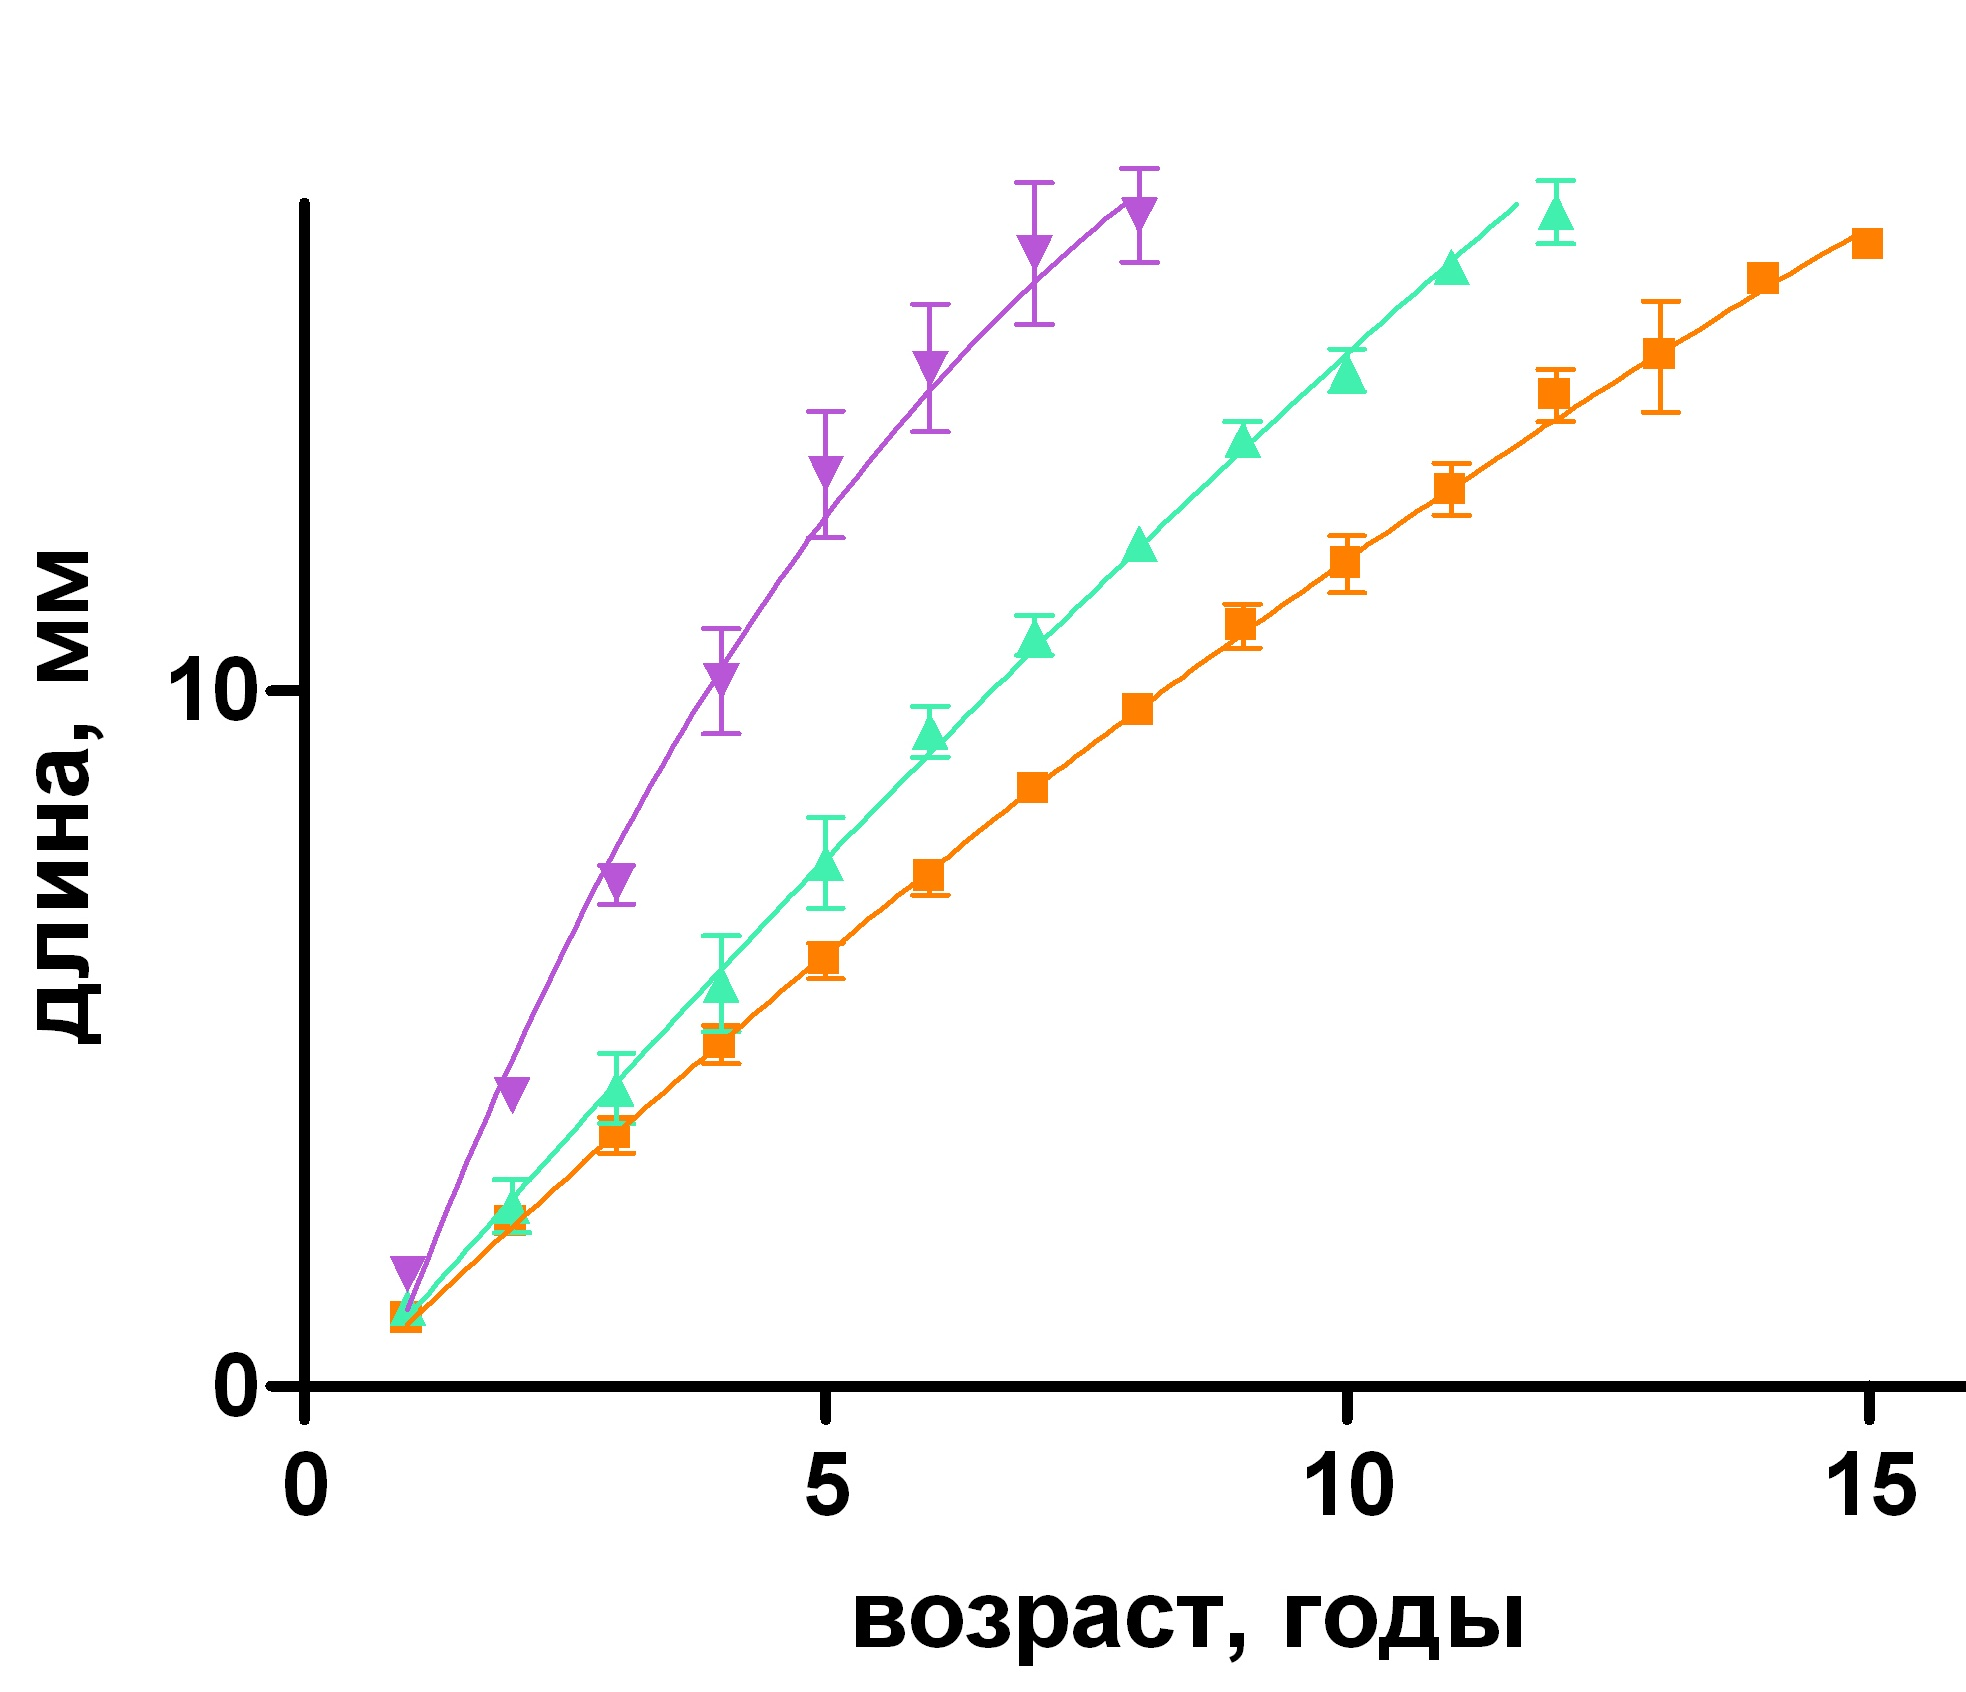
\includegraphics[width=\textwidth]{./rost_clusters_all_crop.jpg}
		\end{center}
	\end{minipage}

1: \textcolor{violet}{Ярнышная СГЛ, Порчниха СГЛ}\\
2: \textcolor{cyan}{Пала СГЛ, Гаврилово СГЛ, Ярнышная ВГЛ, Дальне-Зеленецкая СГЛ, Шельпино СГЛ}\\
3: \textcolor{orange}{Абрам-мыс, Пала НГЛ, Гаврилово СГЛ, Ярнышная НГЛ, Шельпино ВГЛ}
\end{frame}

\begin{frame}{Широтные изменения скорости роста {\it M.~balthica} в европейской части ареала}
{\footnotesize Параметр $\omega = L_{max} \times k$ (Appeldoorn, 1983; Beukema, Meehan, 1985)}
		\begin{center}
			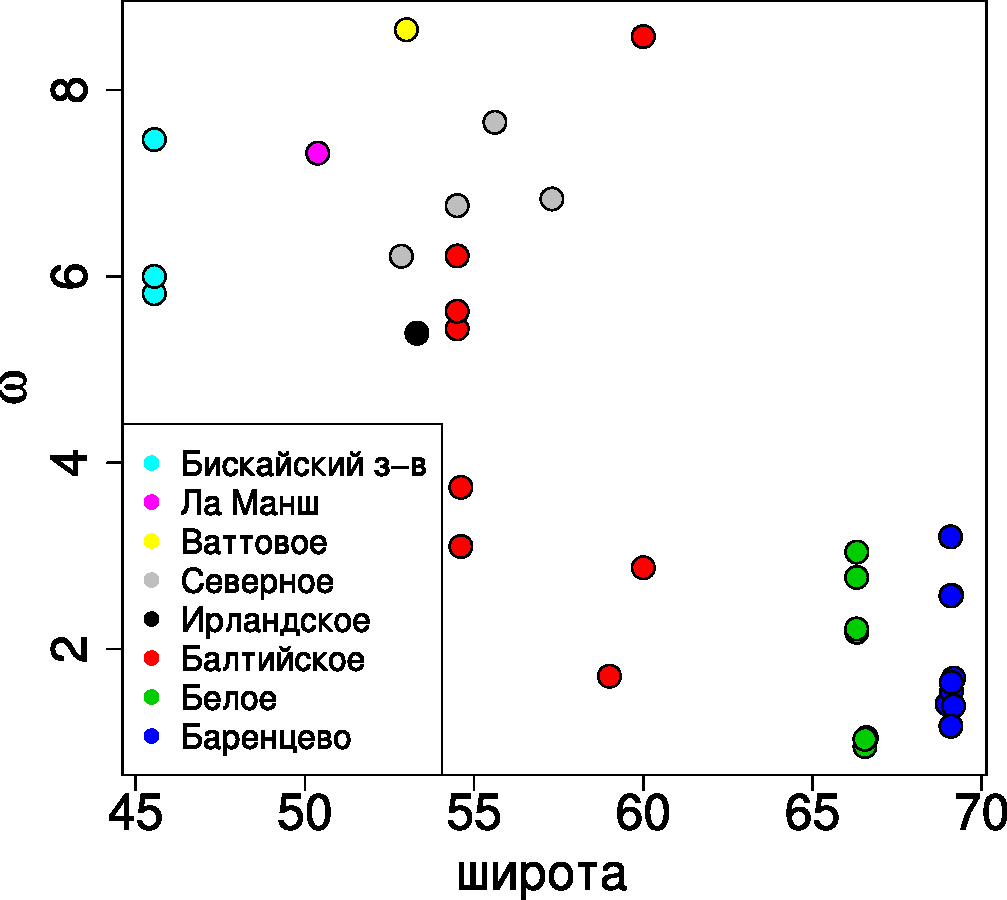
\includegraphics[height=.62\textheight]{./long_vs_omega_big1.pdf}
		\end{center}
{\small Корреляция Спирмена: $r_{s} = -0,60$, $p < 0,0001$.}

\end{frame}

\begin{frame}{Линейный рост {\it M.~balthica} в европейской части ареала}
	\begin{minipage}[t]{.52\linewidth}
		\begin{center}
			\includegraphics[width=\textwidth]{./Europe_clusters_usrednenie.pdf}
		\end{center}

Цветовые обозначения: \textcolor{red}{Баренцево море}, 
\textcolor{blue}{Белое море}, 
\textcolor{cyan}{Балтийское море}, 
\textcolor{green}{Северное море}, 
\textcolor{brown}{Бискайский залив}.
	\end{minipage}
%
	\begin{minipage}[t]{.45\linewidth}
		\begin{center}
			\includegraphics[width=\textwidth]{./Europe_growth_groups_prizm.pdf}
		\end{center}
	\end{minipage}
\end{frame}

%\begin{frame}{\small Изменения среднего годового прироста особей {\it M.~balthica} в зависимости от начальной средней длины их раковин, мареографического уровня обитания (A) и условного смещения участка по побережью Мурмана на восток (Б)}
%	\begin{minipage}[t]{.49\linewidth}
%				{\small А}
%			\begin{center}
%				\includegraphics[width=\textwidth]{./prirost_otklik_mareography.jpg}
%			\end{center}
%		\end{minipage}
%	\hfil %Это пружинка отодвигающая рисунки друг от друга
%		\begin{minipage}[t]{.49\linewidth}
%				{\small Б}
%			\begin{center}
%				\includegraphics[width=\textwidth]{./prirost_otklik_geography.jpg}
%			\end{center}
%		\end{minipage}
%\tiny{1~--- Абрам-мыс, 2~--- Пала-губа, 3~--- Гаврилово, 4~--- Ярнышная, 5~--- Дальнезеленецкая, 6~--- Шельпино, 7~--- Порчниха.\\
%Горизонты литорали: ВГЛ~--- верхний, СГЛ~--- средний, НГЛ~--- нижний.}
%\end{frame}


%%%%%%%%%%%%%%%%%%%%%%%%%%%%%%%%%%%%%%%%%%%%%%%%%%%%%
		\section[Оседание]{Режим формирования спата}
%%%%%%%%%%%%%%%%%%%%%%%%%%%%%%%%%%%%%%%%%%%%%%%%%%%%%
\begin{frame}{Обилие спата \textit{Macoma balthica}}
		\begin{center}
			\includegraphics[width=\textwidth]{N_spat1.pdf}
		\end{center}
\end{frame}



%%%%%%%%%%%%%%%%%%%%%%%%%%%%%%%%%%%%%%%%%%%%%%%%%%%%%
		\section{Выводы}
%%%%%%%%%%%%%%%%%%%%%%%%%%%%%%%%%%%%%%%%%%%%%%%%%%%%%
\begin{small}

\begin{frame}{Выводы}
\addtocounter{enumi}{0}
	\begin{enumerate}
		\item В Кольском заливе Баренцева моря и Кандалакшском заливе  Белого моря значения биомассы (до 200 г/м$^2$) поселений {\it Macoma balthica} сопоставимы с аналогичным показателем в европейской части ареала, а плотность поселений нередко оказывается выше (до 8~тыс.~экз./м$^2$). Для литорали восточной части Мурманского побережья Баренцева моря типичны поселения {\it M.~balthica} с численностью менее 100 экз./м2 
		\item Плотность поселений спата {\it Macoma balthica} в Белом море может варьировать на порядок в пределах незначительной акватории, и достигать десятков тысяч экз./м$^2$.
		\item Беломорские и баренцевоморские поселения {\it M.~balthica} не различаются по средней скорости роста моллюсков, и отличаются по этому показателю минимальными характеристиками в пределах европейской части ареала вида. 
	\end{enumerate}
\end{frame}


\begin{frame}{Выводы}
	\begin{enumerate}
\addtocounter{enumi}{3}
		\item Динамика размерной структуры поселений {\it Macoma balthica} в Белом и Баренцевом представлена двумя типами. \\
Наболее обычный вариант~--- чередование бимодального и мономодального распределений особей по размерам. При этом первый пик формируют молодые
особи (обычно длиной до 5 мм), а второй модальный класс состоит из взрослых особей (в Белом море длиной 9--12~мм, в Баренцевом море~--- 10--17~мм).
Как относительно редкое событие наблюдается мономодальная структура поселений с ежегодным преобладаем молоди.
		\item Динамика плотности поселений {\it Macoma balthica} в Кандалакшском заливе Белого моря демонстрирует элементы синхронности в поселениях, расположенных на расстоянии от 1 до 100~км, что происходит на фоне резкой межгодовой неравномерности пополнения поселений молодью.  
	\end{enumerate}
\end{frame}


\end{small}

		\section*{Благодарности}
\begin{footnotesize}
\begin{frame}{Благодарности}
	\begin{itemize}
\begin{multicols}{2} [\item научному руководителю Н.\:В.~Максимовичу]

		\item{Д.\:А.~Аристову} 
		\item{Е.\:А.~Генельт-Яновскому}
		\item{А.\:В.~Герасимовой}
		\item{М.В.~Иванову}
		\item{И.\:А.~Коршуновой}
		\item{М.\:В.~Макарову}
		\item{С.\:В.~и С.\:С.~Малавендам}
		\item{А.\:Д.~Наумову}
		\item{А.\:В.~Полоскину}
		\item{И.\:П.~Прокопчук}
		\item{П.\:П.~Стрелкову}
		\item{Ю.\:Ю.~Тамберг}
		\item{О.\:С.~Тюкиной}
		\item{В.\:М.~Хайтову}
		\item{К.\:В.~Шунькиной}
		\item{\fbox{Е.\:А. Нинбургу}}
		\item{\fbox{А.\:С.~Корякину}}
		\item{участникам Беломорской экспедиции ГИПС ЛЭМБ}
		\item{участникам студенческой Баренцевоморской экспедиции СПбГУ}
%		\item{участникам Беломорской экспедиции кафедры ихтиологи и гидробиологии СПбГУ}
		\item{администрации Кандалакшского заповедника}
\end{multicols}
	\end{itemize}
{\scriptsize Данная работа частично выполнена при поддержке грантов СПбГУ (1.0.134.2010, 1.42.527.2011, 1.42.282.2012, 1.38.253.2014) и РФФИ (12-04-01507, 13-04-10131К).}
\end{frame}
\end{footnotesize}

\appendix
		\section*{Публикации и апробация работы}
\begin{frame}{Публикации по теме диссертации}
%	\nocite{*}
	%\printbibliography[heading=bibintoc]
%	\printbibliography[env=gostbibliography,sorting=ydnt]
\begin{itemize}
	\item{статьи: 6, из них 3 в журналах из списка ВАК}
		\begin{enumerate}
\begin{footnotesize}
			\item Назарова С.А. и др. Линейный рост \textit{Macoma balthica} в осушной зоне Мурманского побережья Баренцева моря/\textbf{С.А. Назарова}, Е.А.  Генельт-Яновский,  Н.В. Максимович// Вестник СпбГУ, сер.3, вып.4 -- Спб. -- 2010. -- C.~35-43.
\item Genelt-Yanovskiy E. et al Population structure and growth rates at biogeographic extremes: A case study of the common cockle, \textit{Cerastoderma edule} (L.) in the Barents Sea /Eugene Genelt-Yanovsky, Alexey Poloskin, Andrei Granovitch, \textbf{Sophia Nazarova}, Petr Strelkov// Marine Pollution Bulletin. -- Vol. 61, Iss.4-6. -- 2010, P. 247-253 
\item  Nazarova S. et al. Abundance distribution patterns of intertidal bivalves \textit{Macoma balthica} and \textit{Cerastoderma edule} at the Murman coast tidal flats (the Barents Sea)./ \textbf{S.~Nazarova}, E.~Genelt-Yanovsky, K.~Shunkina // Journal of the Marine Biological Association of the United Kingdom., v.~95~(8) -- 2015. — Pp.~1613-1620.
%\item Генельт-Яновский Е.А. и др. Фаунистические комплексы, ассоциированные с поселениями инфаунных двустворчатых моллюсков на литорали Мурманского побережья Баренцева моря/ Е.А.Генельт-Яновский, \textbf{С.А.Назарова}// Материалы VI всероссийской школы по морской биологии "Биоразнообразие сообществ морских и пресноводных экосистем России" (Мурманск, 1-2 ноября 2007 года). -- Мурманск, 2007. -- С.45-46.
%\item Назарова С.А. и др. Структурно-функциональные характеристики поселений \textit{Macoma balthica} L. в осушной зоне Мурманского побережья Баренцева моря/ \textbf{С.А.~Назарова}, Е.А.~Генельт-Яновский//Материалы научной конференции, посвященной 70-летию ББС им. Перцова 9-10 августа 2008 года. -- М., 2008. -- C. 81-85
%\item Генельт-Яновский Е.А. и др. Сообщества илисто-песчаной литорали губы Дальне-Зеленецкая (Восточный Мурман) в 2002-2007 гг/ Е.А.~Генельт-Яновский, \textbf{С.А.~Назарова}//Материалы X научного семинара <<Чтения памяти К.М.~Дерюгина>>. --СПб. -- 2008. -- С.~16-28.
\end{footnotesize}
		\end{enumerate}


	\item{тезисы докладов и материалы конференций: 9}
\end{itemize}
\end{frame}


\begin{frame}{Апробация работы}
\begin{itemize}
	\item{European Marine Biology Symposium: 2011, 2014, 2015}
	\item{Конференция ББС МГУ: 2004, 2008}
	\item{VI всероссийская школы по морской биологии <<Биоразнообразие сообществ морских и пресноводных экосистем России>>: 2007}
	\item{Научная сессия МБС СПбГУ: 2004, 2008, 2009, 2010}
	\item{Дерюгинские чтения: 2008}
	\item{Семинар кафедры ихтиологии и гидробиологии СПбГУ: 2003 -- 2015}
\end{itemize}
\end{frame}

\end{document}

